\documentclass[spanish,nolol,noloa,final,print]{thesis} [2016/07/28 v1.0.3]

\author{Juan Diego Sera Rodr�guez} %en caso de que sean dos poner dos veces el comando \author

\title{OptiChoice Software para el apoyo en la Toma de Decisiones}

\ucicenter{} %en caso que no este vinculado a ningun cenntro dejar en blanco (OJO NO ELIMINAR EL COMANDO, solo dejar \ucicenter{} )

\facultynum{4}

\addtutor[Tutor]{Ing. Luis Manuel Valera} %en caso de m�s de un tutor repetir el comando.
\addtutor[Tutora]{Dr. C. Yamilis Fern�ndez P�rez}

\thought{}
 
\dedicatory{Le dedico este logro a mis padres Juan y Yisell, mi hermana Melissa, mi bisabuela Mam�n y mi abuela Irma, de no ser por ellos nunca hubiese estado donde estoy.\\
	
	A mis t�as y t�os que siempre se preocuparon por mi futuro y bienestar.}

\acknowledgment{Quisiera agradecerle a todas las personas que de una forma u otra me ayudaron a terminar esta etapa de mi vida:\\
	
	Principalmente a mis padres Juan y Yisell y mi hermana los cuales siempre estuvieron ah� para brindarme su apoyo cuando lo necesite.\\
	
	A mi bisabuela Mamin y mi abuela Irma que me criaron como un hijo y siempre han sido mi raz�n de seguir.\\
	
	A mi t�o Ton que aunque no est� conmigo en el plano f�sico se que me sigue apoyando.\\
	
	A mis t�as y mi madrina que siempre ayudaron en lo que pudieron para que no abandonara los estudios.\\
	
	A mis tutores el profesor Luis Manuel y la doctora Yamilis por la dedicaci�n y ayuda prestada durante la realizaci�n de mi tesis.\\
	
	A mis amigos que se han convertido en hermanos Carlos, Danny, Jose, Daniel, Antonio, Fabi�n, y muchos otros que sin ellos realmente no hubiese llegado tan lejos.\\
	
	A Dios que siempre fue mi apoyo para seguir adelante.
	\\
	
	Y a todas las personas que fui conociendo en el camino a lo largo de estos 4 a�os que pusieron su granito de arena aunque ya no sean parte de mi vida actual.}

\abstract{Esta investigaci�n se centra en el desarrollo de un software para el apoyo en la toma de decisiones basado en m�todos de decision multicriterio, con el objetivo de minimizar la subjetividad, mejorar la eficiencia del an�lisis, permitiendo el manejo de grandes vol�menes de datos y el an�lisis de sensibilidad.  El estudio surge de la necesidad de contar con una plataforma integrada que permita aplicar y comparar resultados de diferentes m�todos de toma de decisi�n multicriterio de manera eficiente, superando las limitaciones de las herramientas existentes que generalmente implementan un solo m�todo o carecen de capacidades de comparaci�n robustas. El software desarrollado permite la entrada de datos, la ponderaci�n de criterios, la aplicaci�n de m�todos MCDM (como AHP, TOPSIS, PROMETHEE y ELECTRE) y la visualizaci�n de resultados mediante una interfaz gr�fica intuitiva. La investigaci�n se basa en una metodolog�a �gil, espec�ficamente Extreme Programming (XP). Para la validaci�n de OptiChoice se realizaron pruebas de software a nivel de pruebas unitarias y de aceptaci�n, con el objetivo de validar el cumplimiento de los requisitos y garantizar la calidad del sistema. Adem�s se adicionan  pruebas de veracidad con el objetivo de verificar la precisi�n y exactitud de los m�todos implementados, a partir de comparaci�n con los resultados de art�culos cient�ficos. Las conclusiones destacan que el software no solo optimiza los procesos de toma de decisiones, sino que tambi�n ofrece una plataforma flexible y escalable para futuras investigaciones.\\}

\keywords{Apoyo a la TD, M�todos de toma de decisiones multicriterio, Programaci�n Extrema}

\input{Glossary}
\newacronym{UCI}{UCI}{Universidad de las Ciencias Inform�ticas}
\newacronymeng{MCDM}{MCDM}{Del ingl�s Multi Criteria Decision Maker}


\addbibresource{example.bib} %en caso de que modifiquen el nombre del archivo .bib ac� deben de modificar tambien.

\begin{document}
  \maketitle
  
  \introduction
\chapter*{INTRODUCCIÓN}
\addcontentsline{toc}{chapter}{INTRODUCCIÓN}
\markboth{INTRODUCCIÓN}{INTRODUCCIÓN}

La toma de decisiones constituye un proceso cognitivo fundamental que permea múltiples dominios organizacionales, desde la administración de recursos humanos hasta la formulación de estrategias corporativas. Los procesos decisionales contemporáneos se caracterizan por su complejidad inherente, manifestada a través de la presencia de intereses divergentes, la participación de múltiples actores y la necesidad de evaluar factores de naturaleza heterogénea. Esta complejidad se intensifica exponencialmente cuando los decisores enfrentan escenarios que involucran volúmenes considerables de información, alternativas interdependientes y criterios de evaluación múltiples y frecuentemente conflictivos \citep{cinelli2021}. Como establecen Thomas et al. \citep{thomas2023}, los problemas de toma de decisiones complejos requieren la utilización de ecuaciones matemáticas, estadísticas multivariadas y dispositivos computacionales para calcular y estimar soluciones de manera automatizada, evidenciando las limitaciones de los enfoques tradicionales basados únicamente en el juicio humano.

La resolución de problemas decisionales multicriterio implica el procesamiento cognitivo de múltiples dimensiones de información y la integración de juicios de expertos, procesos que frecuentemente exceden las capacidades de procesamiento del sistema cognitivo humano. La literatura científica documenta consistentemente que el juicio intuitivo presenta limitaciones sistemáticas en contextos de alta complejidad, siendo susceptible a sesgos cognitivos, efectos de anclaje y errores de confirmación que comprometen la objetividad del análisis \citep{berthet2021}. \citep{fugener2021} demuestran que la toma de decisiones estratégicas se ve particularmente afectada por recursos cognitivos limitados, especialmente en escenarios caracterizados por alta incertidumbre y retroalimentación demorada. Investigaciones recientes evidencian que los sistemas de soporte automatizados superan consistentemente a los predictores humanos en tareas de juicio multivariado \citep{rahim2023}, estableciendo así la fundamentación científica para la implementación de Tecnologías de la Información y las Comunicaciones (TIC) como herramientas de apoyo decisional en contextos organizacionales complejos.

En las últimas décadas, los métodos de Toma de Decisiones Multicriterio \ac{MCDM} han experimentado un crecimiento exponencial en su adopción y desarrollo, consolidándose como herramientas analíticas fundamentales para abordar problemas decisionales de alta complejidad \citep{thomas2023}. Estos métodos proporcionan marcos metodológicos estructurados que permiten la descomposición sistemática de problemas multidimensionales, facilitando la evaluación simultánea de criterios heterogéneos —cuantitativos y cualitativos— y la identificación de alternativas óptimas dentro de espacios de decisión complejos \citep{cinelli2021}. La literatura científica documenta más de 10,000 publicaciones en el período 2012-2022, evidenciando su aplicabilidad transversal en dominios que abarcan desde la ingeniería y las finanzas hasta la gestión ambiental y la planificación estratégica organizacional \citep{thomas2023}. 

No obstante, la implementación manual de estos métodos presenta limitaciones sistemáticas bien documentadas que comprometen su efectividad práctica. Entre estas limitaciones se identifican: (i) la introducción de sesgos cognitivos inherentes al procesamiento humano que afectan la consistencia de las evaluaciones \citep{berthet2021}, (ii) la incapacidad para procesar eficientemente matrices de decisión de alta dimensionalidad que caracterizan problemas reales, (iii) las dificultades para mantener la coherencia en comparaciones pareadas cuando el número de criterios y alternativas se incrementa exponencialmente, y (iv) la ausencia de mecanismos automatizados para el tratamiento de información imprecisa, incompleta o caracterizada por incertidumbre epistémica. Estas limitaciones fundamentan la necesidad imperativa de desarrollar plataformas tecnológicas especializadas que automaticen los procesos computacionales subyacentes, preservando la rigurosidad metodológica mientras superan las restricciones cognitivas del análisis manual.

La revisión de la literatura científica acerca de la solución a problemas de toma de decisión con múltiples criterios y experto a permitido identificar los siguientes elementos:

\begin{itemize}
	\item Existencia de múltiples métodos para solucionar este tipo de problemas (ANP, AHP, PROMETHEE, TOPSIS, entre otros)
	\item No existen plataformas flexibles que permitan la comparación de resultados obtenido con diferentes métodos
	\item Muchas de las herramientas existentes son costosas, difíciles de usar o no permiten la integración de múltiples métodos MCDM.
	\item Los métodos manuales de toma de decisiones son propensos a errores, subjetividad y sesgos cognitivos.
\end{itemize}

Dada la \textbf{situación problemática}, se formula el siguiente \textbf{problema a resolver}:

\begin{quote}
	\textit{¿Cómo contribuir a la toma de decisiones usando múltiples criterios en diferentes ámbitos profesionales con la ayuda de las Tecnologías de la Información y la Comunicación?}
\end{quote}

El \textbf{objeto de estudio} serían los Métodos de Decisión Multicriterio y el \textbf{campo de acción} Software de apoyo a la toma de decisiones multicriterio.

El \textbf{objetivo general} de esta investigación es desarrollar un software de apoyo a la toma de decisiones basado en los métodos de toma de decisión multicriterio.

Para lograr este objetivo, se han definido los siguientes \textbf{objetivos específicos}:

\begin{enumerate}
	\item Caracterizar los métodos MCDM más utilizados en la toma de decisiones.
	\item Realizar el análisis de los software homólogos para obtener  las carencias existentes en la industria. 
	\item Elaborar una propuesta de Software que incluya la selección de las herramientas, marcos de trabajo, lenguaje de programación así como el análisis y diseño utilizando una metodología de desarrollo adecuada.
	\item Implementar la propuesta de Software a partir de los artefactos elaborados.
	\item Validar el software mediante casos de estudio reales o simulados, comparando los resultados con los reportados en la literatura científica.
\end{enumerate}

Para la realización de la problemática anterior se utilizaron los \textbf{métodos de investigación científica}, tanto teóricos como empíricos.

Los métodos teóricos utilizados son:

\begin{itemize}
	\item \textbf{Análisis histórico-lógico}: Este método permite estudiar la evolución de un fenómeno a través del tiempo, estableciendo relaciones entre sus diferentes etapas de desarrollo. Se utilizó para examinar la evolución de los métodos MCDM, identificando tendencias y patrones en su aplicación y desarrollo histórico.
	
	\item \textbf{Análisis-síntesis}: Proceso mental que consiste en descomponer un fenómeno en sus partes constitutivas para estudiarlas de forma aislada (análisis) y luego integrar los resultados para obtener una visión global (síntesis). Este método se aplicó para integrar y resumir la información relevante sobre los diferentes métodos MCDM, sus características y aplicaciones, permitiendo establecer relaciones entre conceptos y generar nuevos conocimientos.
	
	\item \textbf{Modelación}: Permite representar de forma simplificada fenómenos complejos mediante modelos que facilitan su estudio. Se utilizó para desarrollar el modelo matemático que sustenta el software MCDM propuesto, representando adecuadamente las relaciones entre alternativas y criterios.
\end{itemize}

Los métodos Empíricos utilizados son:

\begin{itemize}
	\item \textbf{Observación}: Consiste en la percepción directa y registro sistemático de fenómenos. Se aplicó durante las fases de prueba y validación del software, permitiendo recopilar datos sobre usabilidad y eficacia de la interfaz desde la perspectiva del usuario.
	
	\item \textbf{Revisión documental}: Abarca la recolección, selección y análisis de fuentes bibliográficas. Este método fue fundamental para construir el estado del arte y fundamentar teóricamente la investigación, proporcionando una base sólida para el diseño e implementación del software propuesto.
\end{itemize}

El documento se encuentra estructurado en introducción, tres capítulos, conclusiones, recomendaciones, referencias bibliográficas y los anexos.

El \textbf{primer capítulo} se titula ``Fundamentos y Referentes sobre los Software de Toma de Decisiones'' y tiene como objetivo principal analizar los elementos teóricos base de la investigación. Los conceptos esenciales relacionados con toma de decisión multicriterio. Además, posee una descripción de los métodos que resuelven problemas de toma de decisión, así como una breve caracterización de software existentes que dan solución al problema planteado. Se destacarán las herramientas, metodologías y lenguajes de programación que se van a utilizar en el desarrollo del sistema.

El \textbf{segundo capítulo} se titula ``Análisis y diseño de la propuesta de Software OptiChoice'', su objetivo principal es presentar la propuesta de software para la solución de problemas de toma de decisión con múltiples criterios y expertos. Este capítulo contiene los principales elementos que caracterizan la propuesta de solución. Se especifican las características y funcionalidades del sistema como los patrones de diseño y arquitectura a utilizar en el sistema entre otros elementos necesarios para concretar la propuesta, todo esto teniendo en cuenta los requisitos funcionales y no funcionales identificados.

El \textbf{tercer y último capítulo} titulado ``Implementación y Validación de la propuesta de Software OptiChoice'' consiste en presentar los resultados de la implementación y pruebas realizadas a la aplicación. Se describe el proceso de construcción de la plataforma software, así como las pruebas unitarias y de aceptación para validar su correcta elaboración y funcionamiento. Además de la realización de pruebas de veracidad a partir de artículos científicos para demostrar la confiabilidad del software.


  \chapter{Fundamentos y Referentes sobre los Software de Toma de Decisiones}
\label{chap:chapter1}

La toma de decisiones en entornos complejos requiere herramientas especializadas que permitan evaluar m�ltiples criterios de manera objetiva. En este cap�tulo se presentan los fundamentos te�ricos de la toma de decisiones multicriterio (\ac{MCDM}), se analizan los m�todos m�s utilizados en la industria y se examina el estado del arte en software especializado. El objetivo es establecer la base conceptual que justifica el desarrollo de una soluci�n inform�tica optimizada para mejorar los procesos de decisi�n.

\section{La toma de decisiones en problemas complejos con m�ltiples criterios}

La toma de decisiones en problemas complejos es un proceso que involucra la evaluaci�n de m�ltiples alternativas bajo la consideraci�n de varios criterios, a menudo conflictivos entre s� \citep{cinelli2021, steyvers2024}. Estos problemas se caracterizan por su alta dimensionalidad, es decir, la presencia de un gran n�mero de variables, criterios y alternativas, lo que dificulta su resoluci�n mediante m�todos tradicionales \citep{keeney1993, roy1996, berthet2021}.

\subsection{Proceso de toma de decisiones}

El proceso de toma de decisiones es una actividad fundamental en diversos �mbitos, desde la gesti�n empresarial hasta la planificaci�n estrat�gica en organizaciones \citep{simon1960, ali2023}. Este proceso implica seleccionar una alternativa entre varias opciones disponibles, bas�ndose en un an�lisis sistem�tico de los criterios relevantes. En contextos complejos, donde intervienen m�ltiples factores y \textit{stakeholders}, el proceso de toma de decisiones adquiere una mayor relevancia y requiere un enfoque estructurado \citep{freeman1984}.

Este proceso puede dividirse en varias etapas:

\begin{enumerate}
	\item \textbf{Identificaci�n del Problema}: El primer paso es reconocer y definir claramente el problema que requiere una decisi�n. Esto implica entender el contexto, los objetivos y las limitaciones mediante enfoques estructurados que consideren la complejidad inherente de los sistemas modernos \citep{sharma2023}.
	
	\item \textbf{Recopilaci�n de Informaci�n}: Una vez definido el problema, se recopila informaci�n necesaria para evaluar las alternativas. Esto incluye datos cuantitativos y cualitativos, utilizando tecnolog�as avanzadas de an�lisis de datos y sistemas de informaci�n integrados \citep{zhang2024}.
	
	\item \textbf{Generaci�n de Alternativas}: Se identifican las posibles soluciones o alternativas al problema, empleando t�cnicas modernas de creatividad y an�lisis sistem�tico \citep{liu2023}.
	
	\item \textbf{Evaluaci�n de Alternativas}: Las alternativas se eval�an en funci�n de los criterios definidos usando m�todos multicriterio (\ac{MCDM}) para ponderar y comparar las opciones \citep{roy1996}.
	
	\item \textbf{Selecci�n de la Mejor Alternativa}: Se selecciona la alternativa que mejor satisface los criterios y objetivos \citep{keeney1993}.
	
	\item \textbf{Implementaci�n y Seguimiento}: Se implementa la alternativa seleccionada y se monitorean los resultados mediante sistemas de seguimiento en tiempo real \citep{chen2024}.
\end{enumerate}

Los problemas de decisi�n suelen involucrar criterios diversos que pueden ser conflictivos entre s�, como costos, calidad, eficiencia y sostenibilidad. La dificultad radica en equilibrar estos criterios para seleccionar la mejor alternativa posible.

\subsection{Naturaleza de la toma de decisiones en entornos con m�ltiples criterios}

La toma de decisiones en entornos con m�ltiples criterios implica la evaluaci�n de diversas alternativas considerando factores que pueden ser tanto cuantitativos como cualitativos \citep{roy1996}. Para estructurar un problema de decisi�n multicriterio, es fundamental definir los elementos clave:

\begin{itemize}
	\item \textbf{Alternativas (A)}: Conjunto de opciones entre las cuales se debe seleccionar: $A = \{a_1, a_2, a_3, \ldots, a_m\}$ \citep{keeney1993}.
	
	\item \textbf{Criterios (C)}: Factores que influyen en la evaluaci�n de las alternativas: $C = \{c_1, c_2, c_3, \ldots, c_n\}$ \citep{taherdoost2023}.
	
	\item \textbf{Ponderaciones (W)}: Asignaci�n de importancia relativa a cada criterio: $W = \{w_1, w_2, w_3, \ldots, w_n\}$ \citep{saaty1980}.
\end{itemize}

Matem�ticamente, una decisi�n multicriterio puede representarse mediante una matriz de decisi�n \textbf{D}, donde cada alternativa $A_{i}$ es evaluada bajo $n$ criterios:

\[
D = \begin{bmatrix}
	d_{11} & d_{12} & \ldots & d_{1n} \\
	d_{21} & d_{22} & \ldots & d_{2n} \\
	\vdots & \vdots & \ddots & \vdots \\
	d_{m1} & d_{m2} & \ldots & d_{mn} \\
\end{bmatrix}
\]

Donde:
\begin{itemize}
	\item $d_{ij}$ representa la evaluaci�n de la alternativa $A_i$ con respecto al criterio $C_{j}$
	\item $m$ es el n�mero de alternativas
	\item $n$ es el n�mero de criterios
\end{itemize}

Los m�todos \ac{MCDM} permiten transformar esta matriz en una representaci�n que facilite la priorizaci�n de alternativas. Algunos de los enfoques m�s utilizados incluyen:

\begin{enumerate}
	\item \textbf{Normalizaci�n de Valores}: Transformar los valores de la matriz a una escala com�n \citep{hwang1981}: 
	\[r_{ij} = \frac{d_{ij}}{\sqrt{\sum_{i=1}^{m} d_{ij}^2}}\]
	
	\item \textbf{Asignaci�n de Pesos}: Los pesos $w_{j}$ se asignan a cada criterio para reflejar su importancia relativa \citep{saaty1980}.
	
	\item \textbf{Agregaci�n de Resultados}: Los valores normalizados y ponderados se combinan para obtener una puntuaci�n global \citep{roy1996}.
\end{enumerate}

\subsection{Retos y dificultades en la toma de decisiones manual}

La toma de decisiones manual en entornos multicriterio presenta diversas dificultades que pueden comprometer la calidad y eficiencia del proceso decisional \citep{steyvers2024, taherdoost2023}. Entre los principales retos se encuentran la subjetividad en la evaluaci�n de criterios, la dificultad en el manejo de grandes vol�menes de datos y la falta de herramientas anal�ticas que permitan un an�lisis exhaustivo.

En la Tabla \ref{tab:problemas_manuales} se presenta una comparaci�n de los principales problemas encontrados en la toma de decisiones manual:

\begin{table}[H]
	\centering
	\captionbox{Comparaci�n entre los principales problemas de la toma de decisiones\label{tab:problemas_manuales}}
	{
		\begin{tabular}{|p{3cm}|p{5cm}|p{5cm}|}
			\hline
			\textbf{Problema} & \textbf{Descripci�n} & \textbf{Impacto} \\
			\hline
			Subjetividad & Evaluaci�n basada en percepci�n individual sin validaci�n objetiva & Puede generar decisiones inconsistentes \\
			\hline
			Complejidad matem�tica & Dificultad para realizar c�lculos precisos sin herramientas especializadas & Aumenta la probabilidad de errores \\
			\hline
			Gesti�n de grandes vol�menes & Dif�cil de organizar y analizar cuando hay muchas alternativas y criterios & Retrasa el proceso de toma de decisiones \\
			\hline
			Falta de an�lisis de sensibilidad & Imposibilidad de evaluar c�mo cambios en los datos afectan la decisi�n final & Reduce la robustez de la decisi�n \\
			\hline
		\end{tabular}
	}
\end{table}

\subsection{Beneficios del uso de software para apoyar la toma de decisiones}

El uso de software especializado en la toma de decisiones multicriterio ofrece numerosas ventajas en comparaci�n con los m�todos manuales, optimizando la precisi�n, eficiencia y objetividad en la selecci�n de alternativas \citep{madanchian2024, keenan2024}. Los principales beneficios incluyen:

\begin{itemize}
	\item \textbf{Reducci�n de la subjetividad}: El uso de algoritmos estructurados permite minimizar la influencia de sesgos cognitivos y errores humanos \citep{azhar2021}.
	
	\item \textbf{Automatizaci�n de c�lculos complejos}: M�todos como \ac{AHP}, \ac{TOPSIS} y \ac{ELECTRE} requieren operaciones matem�ticas sofisticadas que un software \ac{MCDM} permite realizar de manera autom�tica \citep{yenugula2024}.
	
	\item \textbf{Gesti�n eficiente de grandes vol�menes de datos}: Las herramientas \ac{MCDM} facilitan el procesamiento y an�lisis de m�ltiples criterios y alternativas \citep{sharma2023dss}.
	
	\item \textbf{An�lisis de sensibilidad}: Un software avanzado permite realizar an�lisis de sensibilidad para evaluar c�mo los cambios en los criterios afectan los resultados \citep{pelissari2022}.
\end{itemize}

En la Tabla \ref{tab:comparacion_metodos} se muestra una comparaci�n entre los m�todos manuales y el uso de software:

\begin{table}[H]
	\centering
	\captionbox{Comparaci�n entre m�todos manuales y uso de software\label{tab:comparacion_metodos}}
	{
		\begin{tabular}{|p{3cm}|p{5cm}|p{5cm}|}
			\hline
			\textbf{Aspecto} & \textbf{M�todo Manual} & \textbf{Uso de Software MCDM} \\
			\hline
			Precisi�n de c�lculos & Baja, propensa a errores & Alta, con automatizaci�n total \\
			\hline
			Tiempo de procesamiento & Elevado & R�pido y eficiente \\
			\hline
			Manejo de m�ltiples criterios & Limitado & Ilimitado, soporta grandes vol�menes \\
			\hline
			An�lisis de sensibilidad & Dif�cil de realizar & Integrado y automatizado \\
			\hline
			Generaci�n de reportes & Manual y tedioso & Autom�tica y estructurada \\
			\hline
		\end{tabular}
	}
\end{table}

\section{M�todos de Toma de Decisiones Multicriterio (MCDM)}

Los m�todos de toma de decisiones multicriterio proporcionan un marco anal�tico estructurado para evaluar y seleccionar alternativas en funci�n de m�ltiples criterios \citep{sahoo2023, taherdoost2023}. Estos m�todos han sido ampliamente utilizados en diversas �reas como la ingenier�a, la econom�a, la planificaci�n estrat�gica y la gesti�n de recursos.

Los \ac{MCDM} pueden clasificarse en dos grandes categor�as:

\begin{itemize}
	\item \textbf{M�todos de compensaci�n}: Permiten la sustituci�n de un criterio por otro. Ejemplos incluyen \ac{AHP} y \ac{TOPSIS} \citep{velasquez2013}.
	
	\item \textbf{M�todos de no compensaci�n}: No permiten compensaciones directas entre criterios. Ejemplos incluyen \ac{ELECTRE} y \ac{PROMETHEE} \citep{guitouni1998}.
\end{itemize}

\subsection{AHP (Analytic Hierarchy Process)}

El Proceso Anal�tico Jer�rquico (\ac{AHP}), desarrollado por Thomas L. Saaty en 1980, es un m�todo de toma de decisiones multicriterio que descompone un problema de decisi�n en una jerarqu�a de criterios y alternativas \citep{saaty1980}. Este m�todo es ampliamente utilizado debido a su capacidad para manejar tanto criterios cuantitativos como cualitativos.

\textbf{Algoritmo AHP:}

\begin{enumerate}
	\item \textbf{Definir la jerarqu�a del problema}: El problema se descompone en una jerarqu�a que incluye objetivo principal, criterios y alternativas.
	
	\item \textbf{Construir matrices de comparaci�n por pares}: Se construyen matrices de comparaci�n por pares para cada nivel de la jerarqu�a usando la escala de Saaty de 1 a 9.
	
	\item \textbf{Calcular los valores propios}: Para cada matriz de comparaci�n, se calculan los valores propios mediante la ecuaci�n:
	\[A \cdot w = \lambda_{\max} \cdot w\]
	donde $A$ es la matriz de comparaci�n, $w$ es el vector de pesos, y $\lambda_{\max}$ es el mayor valor propio.
	
	\item \textbf{Evaluar las alternativas}: Los pesos de los criterios se utilizan para evaluar y priorizar las alternativas.
	
	\item \textbf{Verificar la consistencia}: Se verifica la consistencia mediante el �ndice de consistencia:
	\[CI = \frac{\lambda_{\max} - n}{n - 1}\]
	\[CR = \frac{CI}{RI}\]
	donde $n$ es el n�mero de criterios y $RI$ es el �ndice aleatorio.
\end{enumerate}

Las aplicaciones recientes del m�todo \ac{AHP} incluyen evaluaci�n de tecnolog�as emergentes en manufactura avanzada \citep{halicka2020}, gesti�n de cadenas de suministro post-pandemia \citep{kumar2021}, y selecci�n de sitios para instalaciones de energ�a renovable \citep{mohamed2024}.

\subsection{M�todo TOPSIS}

El m�todo \ac{TOPSIS} (Technique for Order Preference by Similarity to Ideal Solution) selecciona la alternativa m�s cercana a una soluci�n ideal y m�s alejada de una soluci�n anti-ideal \citep{hwang1981}.

\textbf{Algoritmo TOPSIS:}

\begin{enumerate}
	\item \textbf{Normalizar la matriz de decisi�n}: Se normaliza mediante la f�rmula:
	\[r_{ij} = \frac{d_{ij}}{\sqrt{\sum_{i=1}^{m} d_{ij}^2}}\]
	
	\item \textbf{Ponderar la matriz}: Se multiplica cada valor normalizado por el peso correspondiente:
	\[v_{ij} = w_{j} \cdot r_{ij}\]
	
	\item \textbf{Determinar las soluciones ideal y anti-ideal}: Se determinan $v_{j}^{+}$ y $v_{j}^{-}$ para cada criterio.
	
	\item \textbf{Calcular distancias}: Se calculan las distancias euclideas:
	\[d_{i}^{+} = \sqrt{\sum_{j=1}^{n} (v_{ij} - v_{j}^{+})^2}\]
	\[d_{i}^{-} = \sqrt{\sum_{j=1}^{n} (v_{ij} - v_{j}^{-})^2}\]
	
	\item \textbf{Calcular el �ndice de similitud}:
	\[C_{i} = \frac{d_{i}^{-}}{d_{i}^{+} + d_{i}^{-}}\]
	
	\item \textbf{Ordenar las alternativas}: Se ordenan seg�n sus valores de $C_{i}$.
\end{enumerate}

El m�todo \ac{TOPSIS} ha encontrado aplicaciones en evaluaci�n de tecnolog�as emergentes \citep{aloini2024}, sistemas de informaci�n hospitalaria \citep{radenovic2023}, y selecci�n de materiales sostenibles \citep{deloitte2025}.

\subsection{M�todo ELECTRE}

\ac{ELECTRE} (Elimination and Choice Expressing Reality) es una t�cnica que se basa en la superaci�n de alternativas mediante comparaciones par a par \citep{roy1968}.

\textbf{Algoritmo ELECTRE:}

\begin{enumerate}
	\item \textbf{Normalizar la matriz de decisi�n}: Se normaliza igual que en \ac{TOPSIS}.
	
	\item \textbf{Construir matrices de concordancia y discordancia}:
	\[C_{ik} = \sum_{j \in J^{+}} w_{j}\]
	\[D_{ik} = \max_{j \in J^{-}} \left( \frac{d_{kj} - d_{ij}}{\max_{i}(d_{ij}) - \min_{i}(d_{ij})} \right)\]
	
	\item \textbf{Aplicar umbrales}: Se definen umbrales de concordancia $(c)$ y discordancia $(d)$.
	
	\item \textbf{Determinar el ranking final}: Se construye un grafo de dominancia basado en las relaciones de superaci�n.
\end{enumerate}

El m�todo \ac{ELECTRE} ha sido aplicado en planificaci�n energ�tica regional \citep{yakici2023}, gesti�n de proyectos de construcci�n \citep{abastante2023}, y evaluaci�n de desempe�o \ac{ESG} \citep{majdi2023}.

\subsection{M�todo PROMETHEE}

\ac{PROMETHEE} (Preference Ranking Organization Method for Enrichment Evaluations) utiliza funciones de preferencia para comparar alternativas y generar un ranking \citep{behzadian2010}.

\textbf{Algoritmo PROMETHEE:}

\begin{enumerate}
	\item \textbf{Definir funciones de preferencia}: Se establecen funciones para cada criterio.
	\item \textbf{Calcular diferencias de preferencia}: Se calculan las diferencias entre alternativas.
	\item \textbf{Obtener flujos de preferencia}: Se calculan flujos positivos y negativos.
	\item \textbf{Ordenar alternativas}: Se ordenan seg�n sus �ndices de preferencia neta.
\end{enumerate}

Las aplicaciones del m�todo \ac{PROMETHEE} incluyen evaluaci�n de tecnolog�as de generaci�n limpia \citep{praene2023}, optimizaci�n en industrias intensivas en energ�a \citep{morais2024}, y selecci�n de tecnolog�as de almacenamiento energ�tico \citep{iea2024}.

\subsection{Otros m�todos}

En la Tabla \ref{tab:otros_metodos} se presentan otros m�todos importantes para la soluci�n de problemas de toma de decisi�n:

\begin{table}[H]
	\centering
	\captionbox{Otros m�todos para la soluci�n de problemas de toma de decisi�n\label{tab:otros_metodos}}
	{
		\begin{tabular}{|p{4cm}|p{6cm}|p{4cm}|}
			\hline
			\textbf{M�todo} & \textbf{Descripci�n} & \textbf{Referencias} \\
			\hline
			MAUT & Utiliza funciones de utilidad para modelar preferencias & Keeney \& Raiffa (1993) \\
			\hline
			VIKOR & Enfocado en la selecci�n de una alternativa de compromiso & Opricovic \& Tzeng (2004) \\
			\hline
			MACBETH & Basado en comparaciones cualitativas & Bana e Costa \& Vansnick (1994) \\
			\hline
			DEMATEL & Analiza relaciones entre criterios & Gabus \& Fontela (1972) \\
			\hline
			MOORA & Optimizaci�n basada en relaciones & Brauers \& Zavadskas (2006) \\
			\hline
		\end{tabular}
	}
\end{table}

\section{Sistemas de Soporte a la Decisi�n (DSS) con M�ltiples Criterios}

Los Sistemas de Soporte a la Decisi�n (\ac{DSS}) son herramientas computacionales dise�adas para asistir a los tomadores de decisiones en la resoluci�n de problemas complejos y no estructurados \citep{morrison2023}. Estos sistemas combinan datos, modelos anal�ticos y tecnolog�as de visualizaci�n para facilitar la evaluaci�n de alternativas en funci�n de m�ltiples criterios.

\subsection{Caracter�sticas Principales y Clasificaciones de los DSS}

Los \ac{DSS} se distinguen por caracter�sticas clave que los hacen especialmente �tiles en entornos empresariales \citep{kumar2024, cintra2023}:

\begin{enumerate}
	\item \textbf{Interactividad y Flexibilidad}: Los \ac{DSS} permiten a los usuarios interactuar con los datos de manera din�mica \citep{ahmed2024}.
	
	\item \textbf{Accesibilidad para usuarios no t�cnicos}: Est�n dise�ados para ser utilizados por personas sin conocimientos t�cnicos avanzados \citep{akyol2024}.
	
	\item \textbf{Rapidez en el Procesamiento}: Utilizan bases de datos optimizadas y tecnolog�as de procesamiento en tiempo real \citep{zheng2024}.
	
	\item \textbf{Integraci�n de Datos}: Los \ac{DSS} modernos integran datos de m�ltiples fuentes heterog�neas \citep{kumar2024}.
	
	\item \textbf{Personalizaci�n}: Cada usuario tiene acceso a informaci�n personalizada seg�n su rol \citep{morrison2023}.
	
	\item \textbf{An�lisis Hist�rico y Predictivo}: Los \ac{DSS} actuales incorporan algoritmos de aprendizaje autom�tico \citep{wieckowski2023}.
\end{enumerate}

Los \ac{DSS} pueden clasificarse en diferentes tipos:

\begin{itemize}
	\item \textbf{DSS Basados en Datos}: Enfatizan el acceso y manipulaci�n de grandes vol�menes de datos \citep{kumar2024}.
	\item \textbf{DSS Basados en Modelos}: Proporcionan acceso a modelos estad�sticos y de optimizaci�n \citep{cintra2023}.
	\item \textbf{DSS Basados en Conocimiento}: Incorporan inteligencia artificial y sistemas expertos \citep{akyol2024}.
	\item \textbf{DSS Basados en Documentos}: Gestionan informaci�n textual no estructurada \citep{ahmed2024}.
	\item \textbf{DSS de Comunicaci�n}: Facilitan la colaboraci�n entre m�ltiples decisores \citep{morrison2023}.
\end{itemize}

\subsection{An�lisis de sistemas hom�logos}

A continuaci�n se presenta un an�lisis de varios \ac{DSS} utilizados en la actualidad para la toma de decisiones multicriterio:

\textbf{Expert Choice}: Herramienta comercial desarrollada para facilitar la toma de decisiones en entornos empresariales, centrada espec�ficamente en la implementaci�n del m�todo \ac{AHP} \citep{goepel2018implementation}.

\textbf{DECERNS}: Plataforma web comercial desarrollada para el an�lisis multicriterio que integra funciones \ac{SIG} con varios m�todos \ac{MCDM} incluyendo MAVT, \ac{AHP}, \ac{TOPSIS}, \ac{PROMETHEE} y MAUT \citep{yatsalo2015decerns}.

\textbf{Visual PROMETHEE}: Herramienta especializada que implementa la metodolog�a PROMETHEE-GAIA, caracterizada por sus capacidades de visualizaci�n avanzadas \citep{mareschal2023visual}.

\textbf{Super Decisions}: Herramienta que implementa el Proceso Anal�tico Jer�rquico (\ac{AHP}) y el Proceso Anal�tico en Red (\ac{ANP}) \citep{sakarya2023analytic}.

\textbf{D-Sight}: Plataforma comercial basada en \ac{PROMETHEE} y GAIA que integra m�ltiples m�todos \ac{MCDM} \citep{dsight2024}.

En la Tabla \ref{tab:sistemas_homologos} se presenta un resumen de los sistemas estudiados:

\begin{table}[H]
	\centering
	\captionbox{Resumen de los sistemas estudiados\label{tab:sistemas_homologos}}
	{
		\begin{tabular}{|p{2cm}|p{2.5cm}|p{2cm}|p{2cm}|p{2.5cm}|p{2.5cm}|}
			\hline
			\textbf{Sistema} & \textbf{M�todos} & \textbf{Nuevos M�todos} & \textbf{Licencia} & \textbf{Incertidumbre} & \textbf{Sensibilidad} \\
			\hline
			Expert Choice & AHP & No & Comercial & No & S� \\
			\hline
			DECERNS & AHP, TOPSIS, PROMETHEE & S� & Comercial & S� & S� \\
			\hline
			Visual PROMETHEE & PROMETHEE I, II & No & Gratuito & No & B�sico \\
			\hline
			Super Decisions & ANP & No & Comercial & No & Avanzado \\
			\hline
			D-Sight & PROMETHEE, AHP & S� & Comercial & S� & Avanzado \\
			\hline
		\end{tabular}
	}
\end{table}

El an�lisis de los sistemas hom�logos evidencia limitaciones que justifican el desarrollo de una nueva soluci�n: fragmentaci�n en el panorama de herramientas \ac{MCDM}, factor econ�mico como barrera considerable, y ausencia de plataformas verdaderamente integradas para comparaci�n sistem�tica de resultados.

\section{Herramientas, Metodolog�as y Lenguajes de Desarrollo}

Para el desarrollo de la propuesta soluci�n se decidi� crear un sistema basado en una plataforma de software utilizando el lenguaje Python. Las herramientas seleccionadas son:

\textbf{Visual Studio Code}: Se seleccion� como \ac{IDE} debido a que es una herramienta gratuita, ligera y altamente personalizable \citep{hunt2023vscode}. Es compatible con m�ltiples lenguajes de programaci�n y sistemas operativos \citep{martin2023vscode}.

\textbf{Visual Paradigm}: Herramienta \ac{CASE} que brinda un conjunto de ayudas para el desarrollo de programas inform�ticos \citep{sommerville2023software}. Soporta el ciclo de vida completo del proceso de desarrollo de software \citep{fowler2023uml}.

\textbf{Lenguaje UML}: Est�ndar adoptado a nivel internacional para crear esquemas, diagramas y documentaci�n relativa a los desarrolladores de software \citep{pilone2023uml}.

\textbf{Lenguaje Python}: Lenguaje de programaci�n de alto nivel, interpretado y multiprop�sito, conocido por su sintaxis clara y legible \citep{vanrossum2024python}. Es ampliamente utilizado en an�lisis de datos, inteligencia artificial y automatizaci�n \citep{mckinney2024pandas}.

Las principales bibliotecas de Python utilizadas incluyen:

\begin{enumerate}
	\item \textbf{NumPy}: Biblioteca fundamental para la computaci�n cient�fica que proporciona soporte para matrices multidimensionales \citep{harris2023numpy}.
	
	\item \textbf{Pandas}: Ofrece estructuras de datos flexibles para manipulaci�n de datos tabulares \citep{mckinney2024pandas}.
	
	\item \textbf{SciPy}: Complementa a NumPy con funciones adicionales para optimizaci�n y �lgebra lineal \citep{virtanen2023scipy}.
	
	\item \textbf{Matplotlib y Seaborn}: Bibliotecas de visualizaci�n para crear gr�ficos estad�sticos \citep{caswell2023matplotlib}.
	
	\item \textbf{Scikit-learn}: Proporciona herramientas para aprendizaje autom�tico y miner�a de datos \citep{pedregosa2023sklearn}.
\end{enumerate}

\textbf{Metodolog�a XP}

Las metodolog�as de desarrollo de software son un conjunto de procedimientos y t�cnicas para el desarrollo de productos software \citep{pressman2024software, sommerville2023software}. Existen metodolog�as tradicionales que priorizan el control del proceso y metodolog�as �giles que se enfocan en la colaboraci�n con el cliente \citep{dings�yr2023agile}.

Extreme Programming (\ac{XP}) es una metodolog�a �gil centrada en potenciar las relaciones interpersonales como clave para el �xito en el desarrollo de software \citep{beck2023xp}. \ac{XP} se basa en realimentaci�n continua, comunicaci�n fluida, simplicidad y coraje para enfrentar los cambios \citep{shore2023agile}.

La metodolog�a \ac{XP} tiene cuatro fases fundamentales:

\begin{enumerate}
	\item \textbf{Planeaci�n}: Interacci�n con el cliente para descubrir y priorizar los requerimientos del sistema, documentados como historias de usuario \citep{cohn2004}.
	
	\item \textbf{Dise�o}: Solo se dise�an las historias de usuario seleccionadas para la iteraci�n actual, promoviendo dise�o simple y refactoring continuo \citep{beck2023xp, fowler2023refactoring}.
	
	\item \textbf{Desarrollo}: Proceso colaborativo que incluye programaci�n en parejas, integraci�n continua y desarrollo guiado por pruebas \citep{williams2023pair, humble2023continuous, beck2023tdd}.
	
	\item \textbf{Pruebas}: Se implementan pruebas unitarias y de aceptaci�n para validar el funcionamiento del software \citep{crispin2023agile}.
\end{enumerate}

Se decidi� usar esta metodolog�a debido a las ventajas que brindan sus caracter�sticas, como la disminuci�n del tiempo de desarrollo sin afectar la calidad del producto \citep{highsmith2023agile}, y su enfoque en generar poca cantidad de artefactos centrados principalmente en el c�digo \citep{beck2023xp}.

\section*{Conclusiones parciales del cap�tulo}

A partir del an�lisis y el estudio realizado se lleg� a las consideraciones siguientes:

\begin{itemize}
	\item La toma de decisiones en contextos complejos requiere un enfoque estructurado y sistem�tico, especialmente cuando intervienen m�ltiples criterios, alternativas y expertos.
	
	\item Se analizaron los m�todos \ac{AHP}, \ac{TOPSIS}, \ac{ELECTRE} y \ac{PROMETHEE}, determinando que cada uno posee aplicaciones �ptimas espec�ficas seg�n el tipo de problema.
	
	\item Los \ac{DSS} son herramientas esenciales para la implementaci�n de m�todos \ac{MCDM} en entornos pr�cticos, destacando su capacidad para integrar datos, modelos anal�ticos y opiniones de expertos.
	
	\item Para lograr una mayor organizaci�n en el proceso de desarrollo se seleccion� Visual Paradigm como herramienta \ac{CASE}, el lenguaje \ac{UML} para el modelado del sistema y Python como lenguaje de programaci�n.
	
	\item El desarrollo de la propuesta soluci�n requiere el uso de un enfoque �gil, adoptando \ac{XP} como metodolog�a dada su flexibilidad ante el cambio de requisitos y el manejo de riesgos.
\end{itemize}
  \chapter{An�lisis y dise�o de la propuesta de Software OptiChoice}
\label{chap:chapter2}

Este cap�tulo tiene como objetivo principal presentar la modelaci�n del software de apoyo a la decisi�n basado en \ac{MCDM}. Para ello, se emplear�n los artefactos de la metodolog�a de desarrollo seleccionada, los cuales ser�n fundamentales en la estructuraci�n del sistema y en su posterior implementaci�n. Se establecen los requisitos funcionales y no funcionales del sistema con la forma de Historias de Usuario, definiendo sus principales caracter�sticas con el objetivo de garantizar su correcto funcionamiento. Finalmente, se analizan los aspectos clave que influir�n en la construcci�n del software, asegurando su eficiencia, escalabilidad y facilidad de uso.

\section{Descripci�n del problema y modelo matem�tico asociado}

Como se analiz� en el primer cap�tulo, los procesos de toma de decisi�n son de suma importancia en el mundo actual, y la realizaci�n manual de cualquier m�todo que le d� soluci�n a los problemas de este tipo puede convertirse en un proceso engorroso (por la cantidad de informaci�n a manejar) y demorar demasiado tiempo en ejecutarlo (por los c�lculos a realizar) \citep{steyvers2024}. La complejidad y tiempo de soluci�n de estos problemas aumenta considerablemente cuando se tienen m�ltiples criterios y expertos. Existen casos en los que un proceso tiene vinculado vol�menes de informaci�n muy grandes, por lo que realizar el an�lisis del mismo de forma manual puede conllevar a cometer errores que repercutan en la decisi�n de la alternativa m�s adecuada y por tanto en la soluci�n del problema.

Desde un punto de vista matem�tico, un problema \ac{MCDM} puede representarse como un sistema en el que se busca optimizar una funci�n objetivo considerando m�ltiples criterios que pueden ser de naturaleza cuantitativa o cualitativa \citep{vincke1992, zeleny1982}.

El problema \ac{MCDM} se puede expresar formalmente de la siguiente manera \citep{roy1996}:

Sea un conjunto finito de $m$ alternativas $A = \{ a_{1},a_{2},...,a_{m}\}$ y un conjunto de $n$ criterios de evaluaci�n $C = \{ c_{1},c_{2},...,c_{n}\}$, donde cada alternativa $a_{i}$ es evaluada con respecto a cada criterio $c_{j}$ mediante una funci�n de desempe�o $f_{j}(a_{i})$ \citep{keeney1993}. Esto da lugar a una matriz de decisi�n $D$ de dimensi�n $m \times n$:

\[
D = \begin{bmatrix}
	f_{1}(A_{1}) & f_{2}(A_{1}) & \ldots & f_{n}(A_{1}) \\
	f_{1}(A_{2}) & f_{2}(A_{2}) & \ldots & f_{n}(A_{2}) \\
	\vdots & \vdots & \ddots & \vdots \\
	f_{1}(A_{m}) & f_{2}(A_{m}) & \ldots & f_{n}(A_{m})
\end{bmatrix}
\]

Cada criterio puede tener diferentes unidades de medida y escalas, por lo que es com�n aplicar t�cnicas de normalizaci�n para homogeneizar los valores y hacerlos comparables \citep{hwang1981, triantaphyllou2000}.

Existen varios tipos de criterios y funciones de agregaci�n en los problemas de tipo \ac{MCDM}, los cuales podr�an clasificarse en \citep{vincke1992}:

\begin{itemize}
	\item \textbf{Criterios de beneficio (+)}: aquellos cuya maximizaci�n es deseable (ej. rentabilidad, calidad, eficiencia).
	\item \textbf{Criterios de costo (-)}: aquellos cuya minimizaci�n es preferida (ej. costos, tiempos de espera, impacto ambiental).
\end{itemize}

Para sintetizar la informaci�n de m�ltiples criterios en una �nica medida de evaluaci�n, se emplean funciones de agregaci�n \citep{keeney1993}. Una de las m�s utilizadas es la combinaci�n lineal ponderada: 

\[S(A_{i}) = \sum_{j=1}^{n} w_{j} \cdot f_{j}(A_{i})\]

donde $w_{j}$ representa el peso asignado a cada criterio $C_{j}$, con la condici�n de que: 

\[\sum_{j=1}^{n} w_{j} = 1 \text{ si } w_{j} \geq 0\]

Los valores $w_{j}$ pueden ser determinados mediante m�todos como el an�lisis jer�rquico de procesos (\ac{AHP}) o t�cnicas de entrop�a para evitar sesgos en la ponderaci�n \citep{saaty1980}.

Dado que la asignaci�n de pesos a los criterios puede influir significativamente en el resultado, el an�lisis de sensibilidad es una herramienta crucial en la toma de decisiones multicriterio \citep{triantaphyllou2000, ishizaka2011}. Se pueden emplear t�cnicas como:

\begin{itemize}
	\item \textbf{Variaci�n de los pesos} $w_{j}$: Evaluar c�mo cambian los resultados si se modifican los valores de peso \citep{vincke1992}.
	\item \textbf{Simulaci�n de Monte Carlo}: Generar m�ltiples escenarios con distribuciones probabil�sticas para los pesos y evaluar la estabilidad de las soluciones \citep{zeleny1982}.
	\item \textbf{M�todos de perturbaci�n}: Aplicar peque�as alteraciones a la matriz de decisi�n para analizar la robustez del modelo \citep{triantaphyllou2000}.
\end{itemize}

\section{Propuesta soluci�n}

A partir del modelo matem�tico anterior y utilizando las tecnolog�as y las herramientas que nos brindan las \ac{TIC} en la actualidad, se propone implementar un sistema que ayude a dar soluci�n a los problemas de toma de decisi�n bajo m�ltiples criterios. Este sistema cumplir� con un grupo de funcionalidades definidas por Historias de Usuario que permitir�n una f�cil interacci�n de los expertos con el mismo, adem�s de traer considerables mejoras a este tipo de procesos.

La herramienta propuesta permitir� importar los datos de un problema de toma de decisi�n a partir de archivos que pueden ser excels, de tipo \ac{CSV} o \ac{JSON} creados o no por el usuario. Luego de que se carguen los datos del problema en la plataforma se le podr�n realizar cambios al mismo y validar la informaci�n obtenida del archivo en un editor de problemas que dispone el sistema. El usuario puede elegir que m�todo usar o si desea usar varios m�todos para darle soluci�n al problema de toma de decisi�n, puede tambi�n si lo desea una vez tenga su soluci�n realizar comparaciones con otros m�todos y ver cual le da un mejor resultado, y finalmente generar una serie de reportes que le brinda el sistema para analizar cu�l o cu�les son las alternativas adecuadas para darle soluci�n al problema. En la Figura \ref{fig:esquema_solucion} se muestra un esquema de la soluci�n propuesta.

\begin{figure}[H]
	\centering
	\captionbox{Esquema de la propuesta soluci�n\label{fig:esquema_solucion}}
	{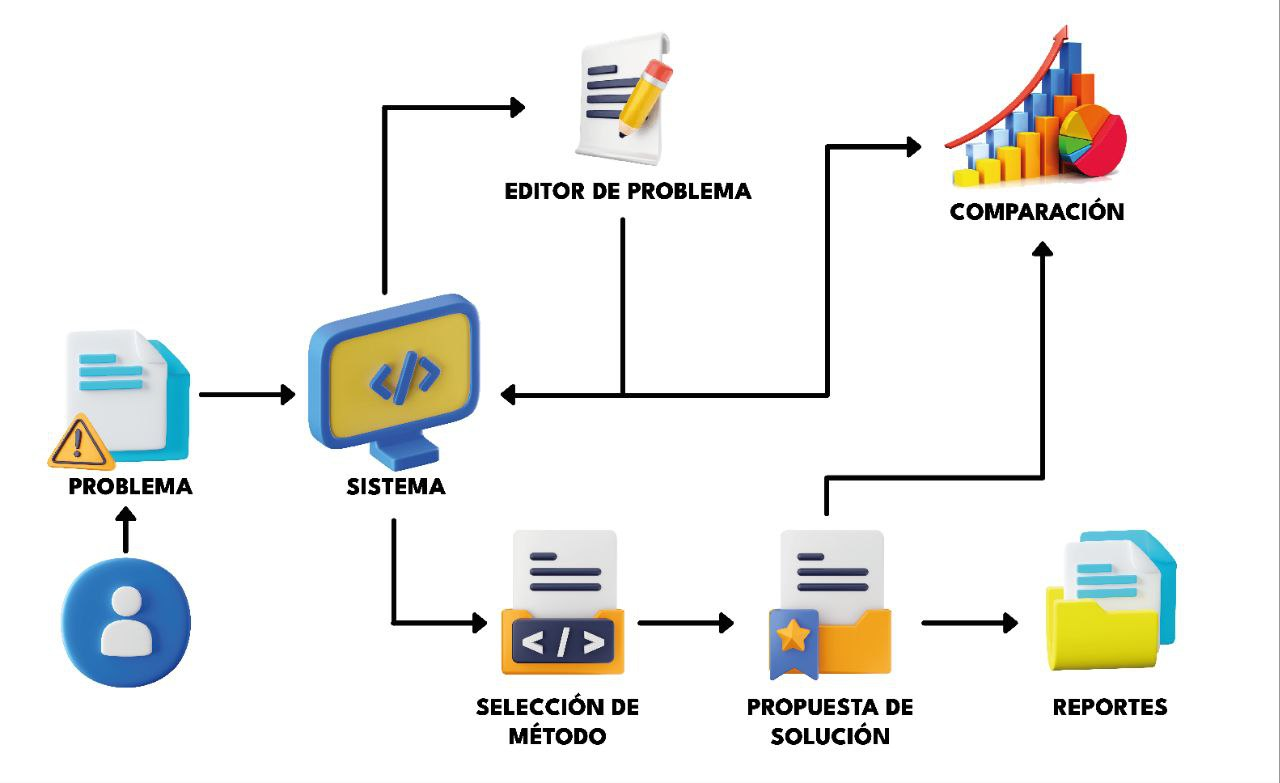
\includegraphics[width=0.7\textwidth]{Anexos/esquema1.jpg}}
\end{figure}

\section{Requisitos del Software}

En la metodolog�a \ac{XP} los requisitos de software est�n dados por las Historias de Usuarios de las cuales se pueden sacar los requisitos funcionales y no funcionales. Los requisitos funcionales son capacidades o condiciones que el sistema debe cumplir sin alterar la funcionalidad del producto. Los requisitos no funcionales son restricciones de los servicios o funciones ofrecidas por el sistema, pueden ser restricciones de tiempo, de los est�ndares a utilizar, de rendimiento, entre otros.

\subsection{Historias de Usuario}

Las Historias de Usuario (\ac{HU}) constituyen uno de los artefactos fundamentales en la metodolog�a de desarrollo \ac{XP}, seleccionada para este proyecto. Representan una t�cnica de especificaci�n de requisitos centrada en el cliente, donde se describen de manera concisa las funcionalidades que el sistema debe implementar. Como se�ala \citep{cohn2004}, estas historias son escritas por el cliente en su propio lenguaje, enfoc�ndose en el valor que aporta cada funcionalidad al negocio sin entrar en detalles t�cnicos de implementaci�n.

Para la identificaci�n de las Historias de Usuario del software \ac{MCDM}, se realizaron reuniones con expertos en toma de decisiones y potenciales usuarios del sistema. En estas sesiones se aplicaron t�cnicas de elicitaci�n de requisitos como entrevistas, tormentas de ideas y an�lisis de escenarios de uso. El resultado fue un conjunto inicial de historias que posteriormente fueron refinadas y priorizadas.

Como indica \citep{cohn2004}, las \ac{HU} deben seguir el principio INVEST (Independent, Negotiable, Valuable, Estimable, Small, Testable), garantizando as� su calidad y viabilidad. Siguiendo este enfoque, cada historia identificada para el software OptiChoice fue evaluada y ajustada para cumplir con estos criterios.

Para el desarrollo del software OptiChoice se identificaron un total de 17 Historias de Usuario, organizadas seg�n las principales funcionalidades del sistema. A continuaci�n, se presentan las m�s relevantes, el resto se puede encontrar en el \hyperlink{historias.usuario.completas}{Anexo de Historias de Usuario}:

% Historia de Usuario 1 - Crear nuevo proyecto de decisi�n
\begin{userstory}[hu:crear_proyecto]
	\storyname{Crear nuevo proyecto de decisi�n}
	\storyuser{Usuario del sistema}
	\storyiter{1}
	\storypriority{Alta}
	\storyrisk{Medio}
	\storypoints{8}
	\storyprogrammer{Juan Diego Sera Rodr�guez}
	\storydescription{
		El sistema permite crear un nuevo proyecto de decisi�n, especificando su nombre, descripci�n y decisor responsable. El proyecto sirve como contenedor para las alternativas, criterios y resultados de los m�todos \ac{MCDM}.
	}
	\storyobservation{
		\begin{itemize}
			\item Debe permitir asignar un nombre �nico al proyecto
			\item Debe almacenar la fecha de creaci�n autom�ticamente
			\item Debe asociar el proyecto a un usuario creador
		\end{itemize}
	}
\end{userstory}

% Historia de Usuario 2 - Gestionar proyectos existentes
\begin{userstory}[hu:gestionar_proyectos]
	\storyname{Gestionar proyectos existentes}
	\storyuser{Usuario del sistema}
	\storyiter{1}
	\storypriority{Media}
	\storyrisk{Medio}
	\storypoints{10}
	\storyprogrammer{Juan Diego Sera Rodr�guez}
	\storydescription{
		El sistema permite listar, buscar, abrir, modificar y eliminar proyectos de decisi�n previamente creados. El usuario puede filtrar proyectos por nombre o fecha de creaci�n.
	}
	\storyobservation{
		\begin{itemize}
			\item Debe mostrar la lista de proyectos con fecha de creaci�n y modificaci�n
			\item Debe permitir b�squedas por nombre o descripci�n
			\item Debe solicitar confirmaci�n antes de eliminar un proyecto
		\end{itemize}
	}
\end{userstory}

% Historia de Usuario 3 - Gestionar alternativas
\begin{userstory}[hu:gestionar_alternativas]
	\storyname{Gestionar alternativas}
	\storyuser{Usuario del sistema}
	\storyiter{1}
	\storypriority{Alta}
	\storyrisk{Medio}
	\storypoints{12}
	\storyprogrammer{Juan Diego Sera Rodr�guez}
	\storydescription{
		El sistema permite a�adir, modificar y eliminar alternativas dentro de un proyecto de decisi�n. Cada alternativa debe tener un identificador �nico, un nombre descriptivo y puede incluir metadatos adicionales.
	}
	\storyobservation{
		\begin{itemize}
			\item Debe validar que el identificador sea �nico dentro del proyecto
			\item Debe permitir a�adir metadatos personalizados a cada alternativa
			\item Debe actualizar la matriz de decisi�n al modificar alternativas
		\end{itemize}
	}
\end{userstory}

% Historia de Usuario 4 - Gestionar criterios de evaluaci�n
\begin{userstory}[hu:gestionar_criterios]
	\storyname{Gestionar criterios de evaluaci�n}
	\storyuser{Usuario del sistema}
	\storyiter{1}
	\storypriority{Alta}
	\storyrisk{Alto}
	\storypoints{16}
	\storyprogrammer{Juan Diego Sera Rodr�guez}
	\storydescription{
		El sistema permite a�adir, modificar y eliminar criterios de evaluaci�n dentro de un proyecto. Cada criterio debe incluir un nombre, tipo de optimizaci�n (maximizar/minimizar), peso y escala (cuantitativa/cualitativa).
	}
	\storyobservation{
		\begin{itemize}
			\item Debe permitir especificar si es un criterio de beneficio o costo
			\item Debe validar que los pesos sean valores positivos
			\item Debe permitir normalizar los pesos autom�ticamente
			\item Debe actualizar la matriz de decisi�n al modificar criterios
		\end{itemize}
	}
\end{userstory}

% Historia de Usuario 5 - Crear matriz de decisi�n
\begin{userstory}[hu:crear_matriz]
	\storyname{Crear matriz de decisi�n}
	\storyuser{Usuario del sistema}
	\storyiter{2}
	\storypriority{Alta}
	\storyrisk{Alto}
	\storypoints{20}
	\storyprogrammer{Juan Diego Sera Rodr�guez}
	\storydescription{
		El sistema permite crear y visualizar una matriz de decisi�n que relacione las alternativas con los criterios establecidos. El usuario puede ingresar los valores de evaluaci�n de cada alternativa respecto a cada criterio.
	}
	\storyobservation{
		\begin{itemize}
			\item Debe mostrar una interfaz tipo tabla con alternativas en filas y criterios en columnas
			\item Debe permitir edici�n directa de valores en la matriz
			\item Debe validar el tipo de datos seg�n la escala del criterio
			\item Debe identificar visualmente el tipo de criterio (beneficio/costo)
		\end{itemize}
	}
\end{userstory}

% Historia de Usuario 6 - Importar datos de matriz de decisi�n
\begin{userstory}[hu:importar_datos]
	\storyname{Importar datos de matriz de decisi�n}
	\storyuser{Usuario del sistema}
	\storyiter{2}
	\storypriority{Media}
	\storyrisk{Alto}
	\storypoints{16}
	\storyprogrammer{Juan Diego Sera Rodr�guez}
	\storydescription{
		El sistema permite importar datos para la matriz de decisi�n desde archivos externos (Excel, \ac{CSV}, \ac{JSON}) facilitando la carga masiva de informaci�n.
	}
	\storyobservation{
		\begin{itemize}
			\item Debe admitir formatos Excel (.xlsx), \ac{CSV} y \ac{JSON}
			\item Debe permitir mapear columnas del archivo con criterios definidos
			\item Debe validar la consistencia de los datos importados
			\item Debe notificar errores espec�ficos durante la importaci�n
		\end{itemize}
	}
\end{userstory}

% Historia de Usuario 7 - Ejecutar m�todo AHP
\begin{userstory}[hu:ejecutar_ahp]
	\storyname{Ejecutar m�todo AHP}
	\storyuser{Usuario del sistema}
	\storyiter{3}
	\storypriority{Alta}
	\storyrisk{Alto}
	\storypoints{24}
	\storyprogrammer{Juan Diego Sera Rodr�guez}
	\storydescription{
		El sistema permite aplicar el m�todo \ac{AHP} (Analytic Hierarchy Process) sobre la matriz de decisi�n, generando matrices de comparaci�n por pares, calculando pesos relativos y verificando la consistencia de los juicios.
	}
	\storyobservation{
		\begin{itemize}
			\item Debe permitir ingresar comparaciones por pares entre criterios
			\item Debe calcular el ratio de consistencia y alertar si supera el umbral (0.1)
			\item Debe calcular el vector de prioridades (eigenvector) para los criterios
			\item Debe generar el ranking final de alternativas seg�n la evaluaci�n \ac{AHP}
		\end{itemize}
	}
\end{userstory}

% Historia de Usuario 8 - Ejecutar m�todo TOPSIS
\begin{userstory}[hu:ejecutar_topsis]
	\storyname{Ejecutar m�todo TOPSIS}
	\storyuser{Usuario del sistema}
	\storyiter{3}
	\storypriority{Alta}
	\storyrisk{Medio}
	\storypoints{16}
	\storyprogrammer{Juan Diego Sera Rodr�guez}
	\storydescription{
		El sistema permite aplicar el m�todo \ac{TOPSIS} (Technique for Order of Preference by Similarity to Ideal Solution) sobre la matriz de decisi�n, calculando las soluciones ideales, distancias y coeficientes de similitud.
	}
	\storyobservation{
		\begin{itemize}
			\item Debe normalizar la matriz de decisi�n seg�n el m�todo seleccionado
			\item Debe calcular las soluciones ideal positiva y negativa para cada criterio
			\item Debe calcular las distancias euclideas y el coeficiente de proximidad relativa
			\item Debe generar el ranking de alternativas seg�n los coeficientes calculados
		\end{itemize}
	}
\end{userstory}

% Historia de Usuario 9 - Visualizar resultados comparativos
\begin{userstory}[hu:visualizar_resultados]
	\storyname{Visualizar resultados comparativos}
	\storyuser{Usuario del sistema}
	\storyiter{4}
	\storypriority{Alta}
	\storyrisk{Alto}
	\storypoints{20}
	\storyprogrammer{Juan Diego Sera Rodr�guez}
	\storydescription{
		El sistema permite visualizar y comparar los resultados obtenidos con diferentes m�todos \ac{MCDM}, mostrando rankings, puntuaciones y diferencias entre m�todos.
	}
	\storyobservation{
		\begin{itemize}
			\item Debe mostrar una vista tabular con rankings por cada m�todo
			\item Debe generar gr�ficos de barras para comparar puntuaciones entre alternativas
			\item Debe calcular y mostrar coeficientes de correlaci�n entre m�todos distintos
			\item Debe identificar gr�ficamente la alternativa �ptima seg�n cada m�todo
		\end{itemize}
	}
\end{userstory}

% Historia de Usuario 10 - Realizar an�lisis de sensibilidad
\begin{userstory}[hu:analisis_sensibilidad]
	\storyname{Realizar an�lisis de sensibilidad}
	\storyuser{Usuario del sistema}
	\storyiter{4}
	\storypriority{Media}
	\storyrisk{Alto}
	\storypoints{24}
	\storyprogrammer{Juan Diego Sera Rodr�guez}
	\storydescription{
		El sistema permite realizar an�lisis de sensibilidad modificando los pesos de los criterios o los valores de la matriz de decisi�n, para evaluar la robustez de los resultados obtenidos.
	}
	\storyobservation{
		\begin{itemize}
			\item Debe permitir modificar interactivamente los pesos de los criterios
			\item Debe recalcular autom�ticamente los resultados al modificar par�metros
			\item Debe generar gr�ficos que muestren c�mo var�a el ranking seg�n cambios en los pesos
			\item Debe calcular indicadores de estabilidad de los resultados
		\end{itemize}
	}
\end{userstory}

Las Historias de Usuario fueron estimadas utilizando el m�todo de Planning Poker, donde el equipo de desarrollo asign� tiempos de implementaci�n basados en la complejidad percibida y la experiencia previa en desarrollos similares. Siguiendo las recomendaciones de \citep{cohn2004}, se consideraron factores como la complejidad t�cnica, el nivel de incertidumbre y la interdependencia entre historias.

\subsection{Plan de Iteraciones}

Las 17 Historias de Usuario identificadas se organizaron en 4 iteraciones de desarrollo, siguiendo un enfoque incremental que prioriza las funcionalidades centrales del sistema:

\textbf{Iteraci�n 1:} Enfocada en la gesti�n b�sica de proyectos, alternativas y criterios (HU 1-4).
\begin{itemize}
	\item HU1: Crear nuevo proyecto de decisi�n
	\item HU2: Gestionar proyectos existentes
	\item HU3: Gestionar alternativas
	\item HU4: Gestionar criterios de evaluaci�n
\end{itemize}

\textbf{Iteraci�n 2:} Centrada en la construcci�n e importaci�n de la matriz de decisi�n (HU 5-8).
\begin{itemize}
	\item HU5: Crear matriz de decisi�n
	\item HU6: Importar datos de matriz de decisi�n
	\item HU11: Validar datos de matriz
	\item HU12: Exportar matriz de decisi�n
\end{itemize}

\textbf{Iteraci�n 3:} Dedicada a la implementaci�n de los m�todos \ac{MCDM} (HU 7-8, 13-15).
\begin{itemize}
	\item HU7: Ejecutar m�todo \ac{AHP}
	\item HU8: Ejecutar m�todo \ac{TOPSIS}
	\item HU13: Ejecutar m�todo \ac{ELECTRE}
	\item HU14: Ejecutar m�todo \ac{PROMETHEE}
	\item HU15: Configurar par�metros de m�todos
\end{itemize}

\textbf{Iteraci�n 4:} Orientada al an�lisis de resultados, visualizaci�n y exportaci�n (HU 9-10, 16-17).
\begin{itemize}
	\item HU9: Visualizar resultados comparativos
	\item HU10: Realizar an�lisis de sensibilidad
	\item HU16: Generar reportes de resultados
	\item HU17: Exportar resultados a formatos externos
\end{itemize}

% Tabla resumen de iteraciones
\begin{effortestimation}[tb:distribucion_hu]
	\addentry[1]{Crear nuevo proyecto de decisi�n}{8} 
	\addentry[1]{Gestionar proyectos existentes}{10} 
	\addentry[1]{Gestionar alternativas}{12} 
	\addentry[1]{Gestionar criterios de evaluaci�n}{16}
	\addentry[2]{Crear matriz de decisi�n}{20} 
	\addentry[2]{Importar datos de matriz de decisi�n}{16} 
	\addentry[2]{Validar datos de matriz}{14} 
	\addentry[2]{Exportar matriz de decisi�n}{12}
	\addentry[3]{Ejecutar m�todo AHP}{24} 
	\addentry[3]{Ejecutar m�todo TOPSIS}{16} 
	\addentry[3]{Ejecutar m�todo ELECTRE}{20} 
	\addentry[3]{Ejecutar m�todo PROMETHEE}{18}
	\addentry[3]{Configurar par�metros de m�todos}{16}
	\addentry[4]{Visualizar resultados comparativos}{20} 
	\addentry[4]{Realizar an�lisis de sensibilidad}{24} 
	\addentry[4]{Generar reportes de resultados}{22}
	\addentry[4]{Exportar resultados a formatos externos}{14}
\end{effortestimation}

Este enfoque de planificaci�n permite entregas incrementales de valor al cliente, siguiendo los principios de \ac{XP}, donde cada iteraci�n produce un incremento funcional del sistema que puede ser evaluado por los usuarios finales.

\section{Tarjetas CRC}

Las tarjetas \ac{CRC} (Clase-Responsabilidad-Colaborador) constituyen un artefacto fundamental en la metodolog�a \ac{XP} para el dise�o de soluciones orientadas a objetos. Tal como se�ala \citep{shore2023agile}, estas tarjetas permiten identificar y organizar las clases que conforman el sistema, sus responsabilidades espec�ficas y las colaboraciones necesarias con otras clases para cumplir dichas responsabilidades.

Durante el an�lisis y dise�o del software \ac{MCDM} propuesto, se identificaron un grupo de clases que aunque no tienen responsabilidades son usadas para contener informaci�n indispensable para el funcionamiento del sistema, estas son Alternative, Criteria, Result y DecisionMatrix. Se defini� tambi�n una clase interfaz MCDMMethodInterface, esta es la clase que debe implementar cada uno de los m�todos de soluci�n que se incluyan en el sistema y contiene las funcionalidades que deben definir los mismos.

A continuaci�n se muestran las tarjetas \ac{CRC} de las clases Project y AHPMethod, el resto de las tarjetas se pueden consultar en el \hyperlink{tarjetas.crc.completas}{Anexo de Tarjetas CRC}:

% Tarjeta CRC de la clase Project
\begin{crccard}[crc:project]
	\crcclass{Project}
	\crcresp
	{
		\begin{itemize}
			\item Crear un nuevo proyecto (Inicializa un proyecto con nombre, descripci�n y decisor)
			\item Adicionar alternativa (Incorpora una nueva alternativa al proyecto)
			\item Adicionar criterio (Incorpora un nuevo criterio de evaluaci�n al proyecto)
			\item Crear matriz de decisi�n (Genera la matriz de evaluaci�n para el proyecto)
			\item Agregar resultado (Almacena el resultado de aplicar un m�todo \ac{MCDM})
			\item Comparar m�todos (Realiza una comparaci�n entre resultados de diferentes m�todos)
			\item Obtener alternativa por ID (Recupera una alternativa espec�fica)
			\item Obtener criterio por ID (Recupera un criterio espec�fico)
			\item Obtener mejor alternativa (Identifica la alternativa con mayor puntuaci�n)
		\end{itemize}
	}
	\crccolab
	{
		Alternative\\
		Criteria\\
		DecisionMatrix\\
		Result
	}
\end{crccard}

% Tarjeta CRC de la clase AHPMethod
\begin{crccard}[crc:ahp_method]
	\crcclass{AHPMethod}
	\crcresp
	{
		\begin{itemize}
			\item Inicializar m�todo (Configura el m�todo \ac{AHP})
			\item Calcular pesos de criterios (Determina la importancia relativa de los criterios)
			\item Calcular prioridades de alternativas (Eval�a alternativas mediante comparaciones)
			\item Calcular pesos desde matriz de comparaci�n (Obtiene eigenvector principal)
			\item Calcular aproximaci�n de pesos (Calcula media geom�trica de filas)
			\item Verificar consistencia (Eval�a la coherencia de las comparaciones)
			\item Ejecutar m�todo (Aplica el algoritmo completo \ac{AHP})
		\end{itemize}
	}
	\crccolab
	{
		MCDMMethodInterface\\
		DecisionMatrix\\
		Result
	}
\end{crccard}

\section{Arquitectura de Software}

La arquitectura de software constituye un elemento esencial en el dise�o de sistemas inform�ticos, representando la estructura fundamental que proporciona una visi�n hol�stica de los componentes del sistema y sus interrelaciones. Seg�n \citep{bass2023software}, la arquitectura de software puede definirse como ``el conjunto de estructuras necesarias para razonar sobre el sistema, que comprende los elementos de software, las relaciones entre ellos y las propiedades de ambos''.

Esta estructura organizativa no solo proporciona un marco para el desarrollo e implementaci�n del sistema, sino que tambi�n establece los lineamientos que determinan sus cualidades de calidad. Como se�ala \citep{gorton2023essential}, una arquitectura bien dise�ada facilita el cumplimiento de requisitos no funcionales como escalabilidad, rendimiento, seguridad y mantenibilidad, mientras optimiza la utilizaci�n de recursos t�cnicos y humanos.

\subsection{Arquitectura N capas}

La arquitectura seleccionada para el software \ac{MCDM} se fundamenta en el modelo de N capas, espec�ficamente estructurado en tres niveles de abstracci�n claramente diferenciados que favorecen la modularidad y el desacoplamiento de responsabilidades. Esta arquitectura, como se�ala \citep{bass2023software}, proporciona una separaci�n l�gica de componentes que facilita el desarrollo, mantenimiento y evoluci�n del sistema, permitiendo que los cambios en un nivel tengan un impacto m�nimo en los dem�s.

La soluci�n desarrollada implementa las siguientes capas, cada una con responsabilidades espec�ficas:

\begin{enumerate}
	\item \textbf{Capa de presentaci�n (Vista)}: Constituye la interfaz con la que interact�a el usuario, incorporando formularios para la definici�n de proyectos, gesti�n de alternativas y criterios, configuraci�n de m�todos y visualizaci�n de resultados. Esta capa est� desarrollada utilizando componentes gr�ficos de Python, espec�ficamente implementados para proveer una experiencia de usuario intuitiva y cohesiva. Los elementos visuales se comunican exclusivamente con la capa de negocio, transmitiendo las solicitudes del usuario y presentando la informaci�n procesada.
	
	\item \textbf{Capa de negocio (Controlador y Aplicaci�n)}: Representa el n�cleo funcional del sistema, donde se implementa la l�gica que procesa las peticiones procedentes de la capa de presentaci�n. Est� conformada por:
	\begin{itemize}
		\item Controladores que coordinan el flujo de informaci�n
		\item Servicios especializados para cada dominio funcional (ProjectService, DecisionService)
		\item Implementaciones de los m�todos \ac{MCDM} (AHPMethod, TOPSISMethod, ELECTREMethod, PROMETHEEMethod)
		\item Validadores que garantizan la integridad de los datos
	\end{itemize}
	
	\item \textbf{Capa de datos (Modelo y Persistencia)}: Gestiona el acceso a datos y la persistencia de la informaci�n, comprendiendo:
	\begin{itemize}
		\item Entidades del dominio (Project, Alternative, Criteria, DecisionMatrix, Result)
		\item Repositorios que abstraen las operaciones de almacenamiento y recuperaci�n
		\item Mecanismos de importaci�n/exportaci�n para diversos formatos (\ac{JSON}, Excel, \ac{CSV}, \ac{PDF})
	\end{itemize}
\end{enumerate}

Esta organizaci�n permite una clara separaci�n entre la interfaz de usuario, la l�gica de negocio y la gesti�n de datos, lo que resulta particularmente beneficioso para un sistema \ac{MCDM} donde los m�todos de an�lisis pueden variar o extenderse sin afectar la experiencia del usuario o la estructura de datos subyacente.

\subsection{Patr�n Arquitect�nico MVC}

El patr�n arquitect�nico Modelo-Vista-Controlador (\ac{MVC}) constituye uno de los fundamentos del dise�o estructural del software \ac{MCDM} propuesto. Este patr�n, como se�ala \citep{pressman2024software}, proporciona una soluci�n demostrada para el problema recurrente de separaci�n de responsabilidades en aplicaciones interactivas, dividiendo el sistema en tres componentes claramente diferenciados.

La implementaci�n del patr�n \ac{MVC} en el sistema de soporte a la decisi�n multicriterio se estructura utilizando un Modelo el cual representa la capa de datos y la l�gica de negocio asociada a la informaci�n del sistema. La vista, la cual constituye la interfaz de usuario que presenta la informaci�n y captura las interacciones, ya sea con formularios, editores, entre otros, y el Controlador que act�a como intermediario entre el modelo y la vista, gestionando el flujo de informaci�n y las operaciones del sistema, en el caso de este trabajo tenemos el MainController como orquestador principal.

\begin{figure}[H]
	\centering
	\captionbox{Patr�n Modelo-Vista-Controlador\label{fig:patron_mvc}}
	{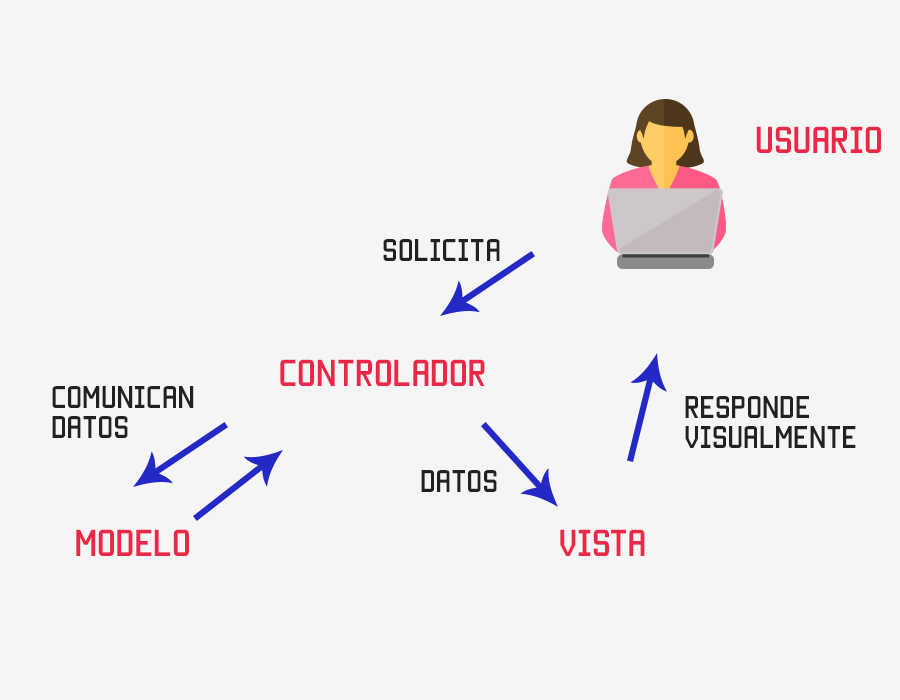
\includegraphics[width=0.7\textwidth]{Anexos/patronmvc.jpg}}
\end{figure}

\section{Patrones de dise�o}

Se considera que en el desarrollo de un sistema inform�tico es de buena pr�ctica utilizar patrones de dise�o, ya que facilitan el trabajo y aportan una mayor organizaci�n y claridad en la estructura de la aplicaci�n. Para el desarrollo del sistema se emplearon los patrones de dise�o en la definici�n de las clases y el dise�o del sistema.

\subsection{Patrones GRASP (Patrones de Software para la Asignaci�n General de Responsabilidad)}

Los patrones \ac{GRASP} (General Responsibility Assignment Software Patterns) constituyen un conjunto de principios fundamentales para la asignaci�n de responsabilidades a clases y objetos en un dise�o orientado a objetos. Como se�ala \citep{larman2023applying}, estos patrones funcionan como gu�as para dise�ar software que sea m�s mantenible, extensible y comprensible. En el desarrollo del software \ac{MCDM} propuesto, se aplicaron varios de estos patrones para garantizar un dise�o robusto.

\subsubsection{Experto en Informaci�n}
El patr�n Experto en Informaci�n sugiere asignar responsabilidades a la clase que posee la informaci�n necesaria para cumplirlas. En nuestra soluci�n, este patr�n se aplic� de forma consistente:

\begin{itemize}
	\item La clase \texttt{DecisionMatrix} encapsula toda la l�gica relacionada con la manipulaci�n de valores de evaluaci�n, incluyendo funciones para obtener y establecer valores, as� como para normalizar la matriz.
	\item Las clases de m�todos \ac{MCDM} (como \texttt{AHPMethod}, \texttt{TOPSISMethod}) contienen los algoritmos espec�ficos para sus respectivos enfoques de evaluaci�n.
	\item La clase \texttt{Project} gestiona la informaci�n relacionada con alternativas, criterios y resultados, siendo responsable de coordinar sus interacciones.
\end{itemize}

\subsubsection{Creador}
El patr�n Creador asigna la responsabilidad de crear instancias de una clase a otra clase. En nuestro sistema:

\begin{itemize}
	\item La clase \texttt{Project} crea instancias de \texttt{DecisionMatrix} mediante el m�todo \texttt{create\_decision\_matrix()}.
	\item \texttt{MCDMMethodFactory} implementa el patr�n Factory para crear instancias de los diferentes m�todos \ac{MCDM}, proporcionando un punto centralizado para la creaci�n de estos objetos.
	\item \texttt{MainController} coordina la creaci�n de proyectos, alternativas y criterios, delegando en los servicios correspondientes.
\end{itemize}

\subsubsection{Controlador}
El patr�n Controlador asigna la responsabilidad de manejar eventos del sistema a clases no vinculadas a la interfaz de usuario. En el software \ac{MCDM}:

\begin{itemize}
	\item \texttt{MainController} act�a como punto de entrada principal para las solicitudes del usuario, coordinando el flujo entre la interfaz y los servicios.
	\item \texttt{ProjectService} y \texttt{DecisionService} proporcionan operaciones especializadas para gestionar proyectos y ejecutar m�todos de decisi�n, respectivamente.
	\item Las clases controladoras no contienen l�gica de presentaci�n ni de dominio, manteniendo una clara separaci�n de responsabilidades.
\end{itemize}

\subsubsection{Alta Cohesi�n}
La Alta Cohesi�n busca mantener las clases enfocadas en un conjunto relacionado de responsabilidades. Este principio se evidencia en:

\begin{itemize}
	\item Las implementaciones de m�todos \ac{MCDM} (como \texttt{AHPMethod} y \texttt{TOPSISMethod}) se concentran exclusivamente en los algoritmos espec�ficos.
	\item El m�dulo de normalizaci�n (\texttt{normalization.py}) agrupa funciones relacionadas con la transformaci�n de datos.
	\item Las entidades del dominio (\texttt{Alternative}, \texttt{Criteria}, \texttt{Result}) encapsulan comportamiento estrechamente relacionado con sus datos.
	\item Los servicios est�n organizados por dominio funcional (proyectos, decisiones) en lugar de por operaciones t�cnicas.
\end{itemize}

\subsubsection{Bajo Acoplamiento}
El Bajo Acoplamiento minimiza las dependencias entre clases, facilitando la modificaci�n y extensi�n del sistema:

\begin{itemize}
	\item La interfaz \texttt{MCDMMethodInterface} permite que la l�gica de ejecuci�n de m�todos no dependa de implementaciones concretas.
	\item La abstracci�n \texttt{ProjectRepository} desacopla el acceso a datos de la l�gica de negocio.
	\item Los servicios como \texttt{DecisionService} interact�an con m�ltiples componentes sin crear dependencias directas entre ellos.
	\item La arquitectura en capas establece l�mites claros de dependencia (presentaci�n ? negocio ? datos).
\end{itemize}

\subsubsection{Polimorfismo}
El principio de Polimorfismo se utiliza para manejar alternativas basadas en el tipo:

\begin{itemize}
	\item Todos los m�todos \ac{MCDM} implementan la interfaz com�n \texttt{MCDMMethodInterface}, permitiendo que sean tratados de manera uniforme.
	\item La estructura de clases para m�todos \ac{MCDM} favorece la extensi�n mediante la adici�n de nuevas implementaciones sin modificar el c�digo existente.
	\item Las operaciones polim�rficas como \texttt{execute()} y \texttt{validate\_parameters()} permiten comportamientos espec�ficos para cada m�todo.
\end{itemize}

\subsubsection{Fabricaci�n Pura}
El patr�n de Fabricaci�n Pura introduce clases que no representan conceptos del dominio pero que proporcionan servicios cohesivos:

\begin{itemize}
	\item \texttt{MCDMMethodFactory} no es un concepto del dominio de decisi�n multicriterio, pero proporciona un servicio cohesivo para la creaci�n y gesti�n de m�todos.
	\item Las clases de utilidades como los validadores (\texttt{AlternativeValidator}, \texttt{CriteriaValidator}) ofrecen servicios de validaci�n sin pertenecer al dominio central.
	\item Los convertidores y normalizadores son fabricaciones puras que encapsulan l�gica t�cnica separada del dominio.
\end{itemize}

\subsubsection{Indirecci�n}
El patr�n de Indirecci�n introduce objetos intermediarios para desacoplar componentes:

\begin{itemize}
	\item Los servicios (\texttt{ProjectService}, \texttt{DecisionService}) act�an como intermediarios entre los controladores y el modelo.
	\item \texttt{FileProjectRepository} proporciona una capa de indirecci�n entre la l�gica de negocio y el sistema de archivos.
	\item Los controladores median entre la interfaz de usuario y los servicios de aplicaci�n.
\end{itemize}

\subsubsection{Variaciones Protegidas}
Este patr�n protege elementos de cambios en otros elementos, encapsulando comportamientos que podr�an variar:

\begin{itemize}
	\item La interfaz com�n para m�todos \ac{MCDM} protege al sistema de cambios en los algoritmos espec�ficos.
	\item Las abstracciones de repositorio protegen la l�gica de negocio de cambios en los mecanismos de persistencia.
	\item La serializaci�n a formatos est�ndar (\ac{JSON}, \ac{CSV}) protege contra cambios en las estructuras de datos internas.
\end{itemize}

La aplicaci�n sistem�tica de estos patrones \ac{GRASP} en el software OptiChoice ha contribuido significativamente a la calidad del dise�o, facilitando la comprensi�n, mantenimiento y extensi�n del sistema. Como resultado, la incorporaci�n de nuevos m�todos \ac{MCDM} o la modificaci�n de los existentes puede realizarse con un impacto m�nimo en el resto del sistema, cumpliendo as� con uno de los requisitos fundamentales identificados durante la fase de an�lisis.

\section*{Conclusiones parciales del cap�tulo}

A partir del an�lisis del sistema se arribaron a las siguientes conclusiones:

\begin{itemize}
	\item El modelado de los procesos de toma de decisiones multicriterio permiti� identificar los subprocesos clave a ser soportados por el sistema: estructuraci�n del problema, construcci�n de matrices, aplicaci�n de m�todos y an�lisis de resultados.
	
	\item La aplicaci�n de la metodolog�a \ac{XP} y la identificaci�n de 17 Historias de Usuario facilitaron la traducci�n efectiva de necesidades del cliente en tareas ingenieriles concretas, organizadas en cuatro iteraciones incrementales.
	
	\item Las tarjetas \ac{CRC} dise�adas reflejan una estructura de clases cohesiva y con bajo acoplamiento, donde cada componente tiene responsabilidades bien definidas, siguiendo los principios de dise�o orientado a objetos.
	
	\item La arquitectura N capas implementada proporciona una clara separaci�n entre presentaci�n, negocio y datos, facilitando el desarrollo independiente de componentes y la incorporaci�n de nuevos m�todos \ac{MCDM}.
	
	\item El patr�n \ac{MVC} refuerza la organizaci�n arquitect�nica, mejorando la mantenibilidad del sistema y separando efectivamente la l�gica matem�tica de la presentaci�n visual.
	
	\item La aplicaci�n sistem�tica de patrones \ac{GRASP} ha mejorado la calidad del dise�o, favoreciendo la alta cohesi�n, el bajo acoplamiento y la extensibilidad del sistema.
	
	\item Las interfaces y abstracciones dise�adas permiten la incorporaci�n de nuevos m�todos \ac{MCDM} sin modificar el c�digo existente, cumpliendo con el requisito de extensibilidad.
	
	\item La propuesta soluci�n implementada soporta adecuadamente criterios de diferentes tipos (beneficio/costo) y escalas, satisfaciendo los requisitos esenciales para un sistema de soporte a la decisi�n.
\end{itemize}
  \chapter{Implementaci�n y Validaci�n de la propuesta de Software OptiChoice}
\label{chap:chapter3}

El presente cap�tulo tiene como objetivo presentar los resultados de la implementaci�n, las pruebas y validaciones realizadas al sistema. Se describen los estilos y est�ndares de implementaci�n utilizados, las pruebas unitarias realizadas al c�digo como pruebas de caja blanca y de aceptaci�n realizadas conjuntamente con el cliente, as� como las validaciones teniendo en cuenta art�culos cient�ficos los cuales se modelaron y solucionaron.

\section{Tareas de Ingenier�a}

Las tareas de ingenier�a constituyen un elemento fundamental en la metodolog�a Extreme Programming (\ac{XP}), ya que permiten descomponer las historias de usuario en actividades t�cnicas concretas y manejables que pueden ser estimadas, priorizadas y completadas dentro de una iteraci�n \citep{cohn2004}. La definici�n de estas tareas proporciona al equipo de desarrollo una comprensi�n clara de los pasos necesarios para implementar cada funcionalidad, facilitando la planificaci�n del trabajo y el seguimiento del progreso \citep{beck2023xp}.

En el contexto del desarrollo del software \ac{MCDM}, las tareas de ingenier�a sirven para \citep{wake2023extreme, shore2023agile}:

\begin{enumerate}
	\item Traducir los requisitos funcionales expresados en las historias de usuario en actividades t�cnicas espec�ficas.
	\item Identificar dependencias t�cnicas entre diferentes componentes del sistema.
	\item Estimar con mayor precisi�n el esfuerzo requerido para cada funcionalidad. 
	\item Facilitar la distribuci�n del trabajo entre los miembros del equipo. 
	\item Establecer criterios claros de completitud para cada historia de usuario.
\end{enumerate}

A continuaci�n, se presenta la tabla que relaciona cada historia de usuario con sus respectivas tareas de ingenier�a, organizadas por iteraci�n. En el \hyperlink{tareas.ingenieria.completas}{Anexo de Tareas de Ingenier�a} se encuentran las especificaciones detalladas:

\begin{longtable}[c]{|p{2cm}|p{5cm}|p{7cm}|}
	\captionsetup{margin=1.15\leftmargin}
	\caption{Tareas de Ingenier�a por Historia de Usuario}
	\label{tab:tareas_ingenieria} \\[2ex]
	
	\hline 
	\rowcolor{gray!25}
	\multicolumn{1}{|c|}{\textbf{Iteraci�n}} & 
	\multicolumn{1}{c|}{\textbf{Historia de Usuario}} & 
	\multicolumn{1}{c|}{\textbf{Tareas de Ingenier�a}} \\ 
	\hline 
	\endfirsthead
	
	\caption{continuaci�n de la p�gina anterior} \\
	\hline 
	\rowcolor{gray!25}
	\multicolumn{1}{|c|}{\textbf{Iteraci�n}} &
	\multicolumn{1}{c|}{\textbf{Historia de Usuario}} &
	\multicolumn{1}{c|}{\textbf{Tareas de Ingenier�a}} \\ 
	\hline 
	\endhead
	
	\hline \multicolumn{3}{|r|}{{Contin�a en la p�gina siguiente}} \\ \hline
	\endfoot
	
	\hline
	\endlastfoot
	
	\multirow{4}{*}{1} & HU1: Crear nuevo proyecto de decisi�n & Implementar entidad Project, ProjectRepository y operaciones CRUD b�sicas \\
	\cline{2-3}
	& HU2: Gestionar proyectos existentes & Desarrollar ProjectService con operaciones CRUD, b�squeda y duplicaci�n \\
	\cline{2-3}
	& HU3: Gestionar alternativas & Implementar entidad Alternative y AlternativeValidator con gesti�n de metadatos \\
	\cline{2-3}
	& HU4: Gestionar criterios de evaluaci�n & Desarrollar entidad Criteria, enums y CriteriaValidator con validaciones completas \\
	\hline
	\multirow{4}{*}{2} & HU5: Crear matriz de decisi�n & Implementar entidad DecisionMatrix con manipulaci�n de arrays NumPy \\
	\cline{2-3}
	& HU6: Importar datos de matriz de decisi�n & Desarrollar funciones de importaci�n para Excel, CSV y JSON \\
	\cline{2-3}
	& HU11: Validar datos de matriz de decisi�n & Implementar MatrixValidator con validaciones de consistencia y completitud \\
	\cline{2-3}
	& HU12: Exportar matriz de decisi�n & Desarrollar funciones de exportaci�n para m�ltiples formatos con ReportLab \\
	\hline
	\multirow{5}{*}{3} & HU7: Ejecutar m�todo AHP & Implementar AHPMethod con eigenvectores y verificaci�n de consistencia \\
	\cline{2-3}
	& HU8: Ejecutar m�todo TOPSIS & Desarrollar TOPSISMethod con soluciones ideales y m�ltiples m�tricas de distancia \\
	\cline{2-3}
	& HU13: Ejecutar m�todo ELECTRE & Implementar ELECTREMethod con matrices de concordancia/discordancia y destilaci�n \\
	\cline{2-3}
	& HU14: Ejecutar m�todo PROMETHEE & Desarrollar PROMETHEEMethod con funciones de preferencia y flujos \\
	\cline{2-3}
	& HU15: Configurar par�metros de m�todos & Implementar MCDMMethodInterface, Factory pattern y m�dulo de normalizaci�n \\
	\hline
	\multirow{4}{*}{4} & HU9: Visualizar resultados comparativos & Implementar entidad Result y DecisionService con comparaciones entre m�todos \\
	\cline{2-3}
	& HU10: Realizar an�lisis de sensibilidad & Desarrollar an�lisis de sensibilidad con variaci�n de pesos y estabilidad de rankings \\
	\cline{2-3}
	& HU16: Generar reportes de resultados & Extender funciones de exportaci�n con reportes detallados y recomendaciones \\
	\cline{2-3}
	& HU17: Exportar resultados a formatos externos & Implementar MainController, API REST con Flask y sistema de excepciones \\
\end{longtable}

Esta estructuraci�n de tareas permite una implementaci�n sistem�tica y controlada del sistema, asegurando que cada componente sea desarrollado, probado e integrado de manera efectiva siguiendo los principios de la metodolog�a \ac{XP} \citep{beck2023xp}.

\section{Est�ndares de Codificaci�n}

Los est�ndares de codificaci�n son reglas y convenciones que se siguen para la escritura del c�digo fuente de un programa. Estos est�ndares aseguran la consistencia, legibilidad y mantenibilidad del c�digo, facilitando el trabajo colaborativo y la evoluci�n del sistema.

\subsection{Nombres de Estructuras}

\textbf{Nombre de las clases:} El estilo de capitalizaci�n utilizado para la notaci�n de las clases es el PascalCase (tambi�n conocido como UpperCamelCase), donde cada palabra que conforma el nombre de la clase comienza con la primera letra en may�sculas. Ejemplos: \texttt{Project}, \texttt{DecisionMatrix}, \texttt{AHPMethod}, \texttt{CriteriaValidator}.

\textbf{Nombre de los m�todos y funciones:} El estilo de nomenclatura utilizado para los m�todos y funciones es el snake\_case, donde las palabras se separan por guiones bajos y todas las letras est�n en min�sculas. Ejemplos: \texttt{execute\_method()}, \texttt{calculate\_weights()}, \texttt{validate\_parameters()}.

\textbf{Nombre de los atributos, par�metros y variables:} Al igual que los m�todos, se utiliza el estilo snake\_case para atributos, par�metros y variables. Para los atributos privados de clase se utiliza un gui�n bajo como prefijo. Ejemplos: \texttt{matrix\_values}, \texttt{weights\_array}, \texttt{\_current\_project}.

\textbf{Nombre de las constantes:} Las constantes se escriben en may�sculas separadas por guiones bajos (UPPER\_CASE). Ejemplos: \texttt{MAX\_ITERATIONS}, \texttt{DEFAULT\_THRESHOLD}, \texttt{RANDOM\_CONSISTENCY\_INDEX}.

\subsection{Reglas de Codificaci�n}

Se definieron las siguientes reglas para garantizar la claridad y consistencia del c�digo:

\begin{itemize}
	\item Utilizar nombres descriptivos y significativos para todas las estructuras, evitando abreviaturas poco claras
	\item No utilizar caracteres simples como nombres de variables, excepto para �ndices en bucles (i, j, k)
	\item Incluir docstrings para todas las clases, m�todos y funciones p�blicas
	\item Mantener l�neas de c�digo de no m�s de 79 caracteres de longitud
	\item Utilizar 4 espacios para la indentaci�n (no tabuladores)
	\item Separar las importaciones en grupos: m�dulos de la biblioteca est�ndar, paquetes de terceros y m�dulos locales
	\item Incluir dos l�neas en blanco entre clases y funciones de nivel superior
	\item Usar espacios alrededor de operadores y despu�s de comas
	\item No usar espacios innecesarios antes de par�ntesis, corchetes o llaves
	\item Documentar los par�metros y valores de retorno de los m�todos usando el formato de docstring de Google
	\item Manejar excepciones de forma espec�fica, evitando cl�usulas except gen�ricas
	\item Usar type hints para mejorar la legibilidad y facilitar la detecci�n de errores
\end{itemize}

\section{Diagrama de Despliegue}

El diagrama de despliegue es un tipo de diagrama estructural \ac{UML} que describe la configuraci�n f�sica del hardware y la distribuci�n del software sobre los nodos de procesamiento. Este diagrama muestra la arquitectura del sistema en tiempo de ejecuci�n, ilustrando las relaciones entre los componentes de hardware y software, as� como las conexiones entre los diferentes nodos del sistema.

\begin{figure}[H]
	\centering
	\captionbox{Diagrama de Despliegue del Sistema OptiChoice\label{fig:deployment_diagram}}
	{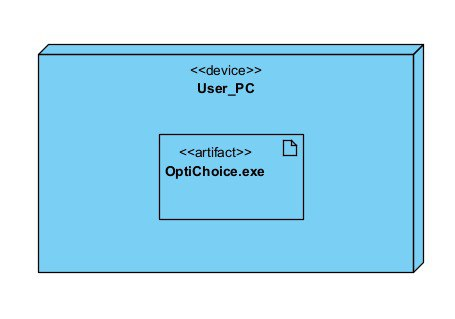
\includegraphics[width=0.7\textwidth]{Anexos/deployment.jpg}}
\end{figure}

\section{Interfaces de la aplicaci�n}

La interfaz principal de la aplicaci�n brinda al usuario la posibilidad de iniciar un nuevo proyecto, agregando informaci�n como nombre del proyecto, descripci�n y quien ser� el encargado de la toma de decisiones, adem�s de poder a�adir, editar y eliminar alternativas y criterios.

\begin{figure}[H]
	\centering
	\captionbox{Interfaz principal del software OptiChoice\label{fig:interfaz_principal}}
	{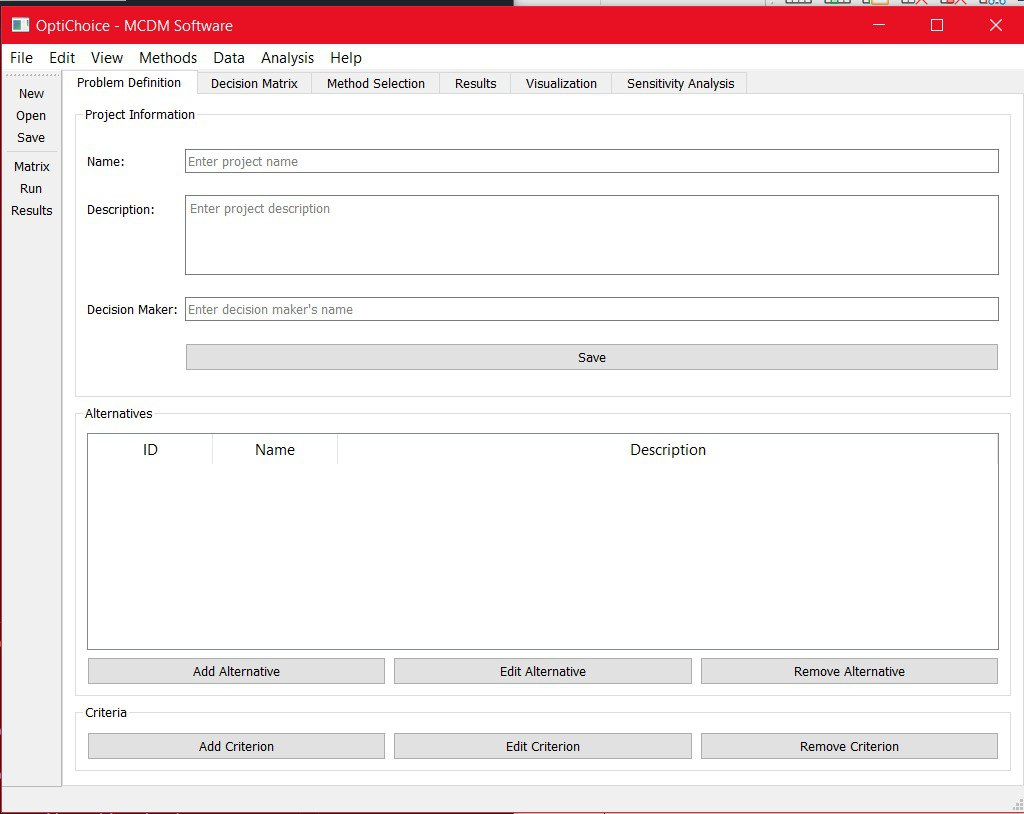
\includegraphics[width=0.6\textwidth]{Anexos/interfaz.jpg}}
\end{figure}

Desde la interfaz principal, presentada en la Figura \ref{fig:interfaz_principal}, el usuario puede crear nuevos proyectos, guardarlos, abrir proyectos existentes y exportar e importar proyectos desde archivos excels, csv o pdf. En el men� ``Methods'' el usuario puede elegir que m�todos desea utilizar en su proyecto e incluso a�adir otros m�todos que no est�n por defecto. M�s detalles sobre las interfaces del sistema se pueden encontrar en el \hyperlink{interfaces.completas}{Anexo de Interfaces}.

\section{Pruebas de Software}

Dentro del proceso de desarrollo de software la fase de pruebas es una de las m�s importantes. El objetivo de esta fase es validar que los requerimientos de software han sido cumplidos, adem�s de garantizar la calidad del sistema.

\subsection{Pruebas Unitarias}

Las pruebas unitarias son dise�adas por los desarrolladores con el objetivo de verificar el c�digo. Estas pruebas se le realizan a las funcionalidades de las clases para obtener los posibles errores que pudieran ocurrir durante su ejecuci�n.

Las pruebas unitarias se realizaron utilizando la librer�a pytest del lenguaje Python. Esta librer�a permite realizar la ejecuci�n de clases Python de manera automatizada y controlada para comprobar si el funcionamiento de las funcionalidades de una clase se comporta de la manera esperada. 

\begin{figure}[H]
	\centering
	\captionbox{Pruebas unitarias a la clase PROMETHEE\label{fig:test_promethee}}
	{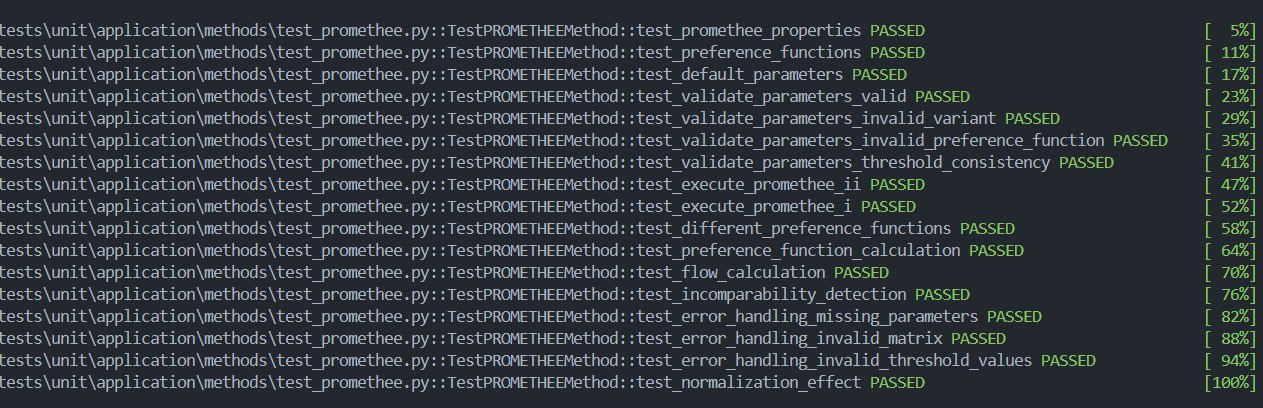
\includegraphics[width=0.7\textwidth]{Anexos/test_promethee.jpg}}
\end{figure}

La Figura \ref{fig:test_promethee} muestra los resultados de las pruebas realizadas a la clase PROMETHEE en las que todas fueron satisfactorias. La prueba fue ejecutada por Juan Diego Sera Rodr�guez y verificada por el Ing. Luis Manuel Valera. Algunas de las otras pruebas realizadas a otras clases se encuentran en el \hyperlink{pruebas.unitarias.completas}{Anexo de Pruebas Unitarias}.

\subsubsection{An�lisis de Resultados}

Luego de haber implementado las historias de usuario planificadas en la primera iteraci�n del desarrollo del sistema \ac{MCDM}, se realiz� la primera iteraci�n de pruebas unitarias detect�ndose treinta y dos no conformidades (\ac{NC}). La mayor parte de estas estaban asociadas a los validadores de entrada de datos (alternativas, criterios y matrices de decisi�n) y a la correcta implementaci�n de los algoritmos \ac{TOPSIS} y \ac{AHP}. Espec�ficamente, se identificaron problemas en el c�lculo de normalizaciones y en el manejo de las matrices de comparaci�n para \ac{AHP}.

Luego de haber implementado las historias de usuario planificadas en la segunda iteraci�n del desarrollo del sistema, corregidas ya todas las \ac{NC} encontradas, se realiz� la segunda iteraci�n de pruebas unitarias detect�ndose dieciocho \ac{NC}. Las inconformidades principales estaban relacionadas con los m�todos \ac{ELECTRE} y \ac{PROMETHEE}, espec�ficamente en el c�lculo de flujos de preferencia y matrices de concordancia/discordancia.

Luego de haber implementado las historias de usuario planificadas en la tercera iteraci�n del desarrollo del sistema y corregidas todas las \ac{NC} encontradas anteriormente, se realiz� una tercera iteraci�n de pruebas unitarias detect�ndose quince \ac{NC}. Estas inconformidades estaban principalmente relacionadas con la integraci�n entre el frontend y el backend.

Luego de ser corregidas las \ac{NC} detectadas en la tercera iteraci�n, se realiz� una cuarta iteraci�n de pruebas unitarias detect�ndose ocho \ac{NC} menores relacionadas con la visualizaci�n de resultados en el frontend. Posteriormente a la correcci�n de estas �ltimas inconformidades, se realiz� una quinta y �ltima iteraci�n de pruebas unitarias en la que no se detectaron \ac{NC}, obteniendo un resultado satisfactorio. Se realiz� un total de cinco iteraciones de pruebas unitarias.

El resultado de las pruebas unitarias en cada iteraci�n se puede apreciar en la Figura \ref{fig:analisis_pruebas_unitarias}.

\begin{figure}[H]
	\centering
	\captionbox{Resultado de las pruebas unitarias por iteraci�n\label{fig:analisis_pruebas_unitarias}}
	{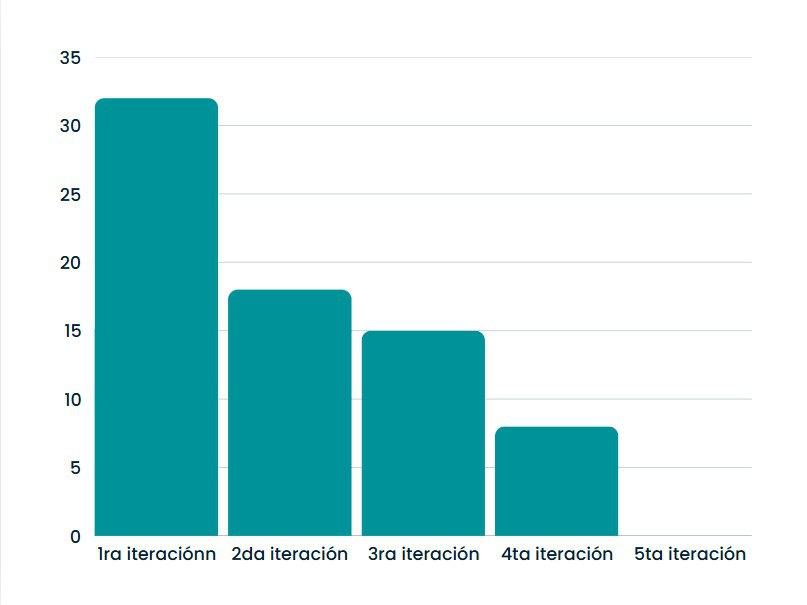
\includegraphics[width=0.7\textwidth]{Anexos/analisis1.jpg}}
\end{figure}

\subsection{Pruebas de Aceptaci�n}

Las pruebas de aceptaci�n son las encargadas de validar el nivel de satisfacci�n del cliente con el software desarrollado, por lo que el cliente tiene la responsabilidad de verificar que los resultados de estas pruebas sean correctos. Estas pruebas constituyen la �ltima verificaci�n antes de la entrega final del software, asegurando que el sistema cumple con todos los requisitos funcionales y no funcionales especificados por el cliente.

Durante el desarrollo del sistema \ac{MCDM}, se realizaron m�ltiples pruebas de aceptaci�n para cada historia de usuario implementada. A continuaci�n, se muestra la prueba de aceptaci�n realizada a una de las historias de usuario m�s cr�ticas del sistema: la ejecuci�n del m�todo \ac{TOPSIS}. El resto de las pruebas de aceptaci�n realizadas al sistema se encuentran detalladas en el \hyperlink{pruebas.aceptacion.completas}{Anexo de Pruebas de Aceptaci�n}.

% Prueba de aceptaci�n del m�todo TOPSIS
\begin{acceptancetest}[pa:ejecutar_topsis]
	\testcasecode{HU8\_P1}
	\testcasedescription{Prueba de funcionalidad para ejecutar el m�todo \ac{TOPSIS} sobre una matriz de decisi�n previamente definida.}
	\testcaseexeccond{
		- Debe existir un proyecto creado\\
		- Deben estar definidas las alternativas y criterios\\
		- Debe estar completada la matriz de decisi�n
	}
	\testcaseexecstep{
		- El usuario selecciona la pesta�a ``M�todos''\\
		- Elige el m�todo \ac{TOPSIS} de la lista\\
		- Configura los par�metros del m�todo (tipo de normalizaci�n, m�trica de distancia)\\
		- Presiona el bot�n ``Ejecutar''\\
		- El sistema procesa la matriz y aplica el algoritmo \ac{TOPSIS}
	}
	\testcaseexpresult{Se muestran los resultados del m�todo \ac{TOPSIS} incluyendo: ranking de alternativas, scores, matriz normalizada y distancias a las soluciones ideales.}
	\testcasename{Ejecutar m�todo TOPSIS}
	\testcaseuserstory{8}
\end{acceptancetest}

\subsubsection{An�lisis de los Resultados}

En las pruebas de aceptaci�n se realizaron cinco iteraciones. Una vez implementadas las historias de usuario de la primera iteraci�n del desarrollo del sistema, se realiz� la primera iteraci�n de las pruebas de aceptaci�n, detect�ndose quince no conformidades; de estas, seis estaban relacionadas con la gesti�n de proyectos (creaci�n, edici�n y eliminaci�n), cuatro con la definici�n de alternativas y criterios, y las cinco restantes con la creaci�n de matrices de decisi�n.

Despu�s, una vez implementadas las historias de usuario de la segunda iteraci�n y corregidas las no conformidades detectadas en la iteraci�n anterior, se desarroll� la segunda iteraci�n de pruebas de aceptaci�n detect�ndose ocho no conformidades relacionadas con la ejecuci�n correcta de los m�todos \ac{TOPSIS} y \ac{AHP}. Espec�ficamente, los problemas estaban vinculados con la normalizaci�n de matrices y el c�lculo de pesos en el m�todo \ac{AHP}.

Luego de corregidas las no conformidades de la segunda iteraci�n de prueba e implementadas las historias de usuario de la tercera iteraci�n, se realiz� la tercera iteraci�n de las pruebas de aceptaci�n, detect�ndose cinco no conformidades relacionadas con la visualizaci�n de resultados y generaci�n de gr�ficos comparativos. Adicionalmente, se encontraron dos problemas con la exportaci�n de resultados a formatos \ac{PDF} y Excel.

Posteriormente, corregidas las no conformidades de la tercera iteraci�n y desarrolladas las historias de usuario de la cuarta iteraci�n, se procedi� a realizar la cuarta iteraci�n de pruebas de aceptaci�n detect�ndose tres no conformidades relacionadas con el an�lisis de sensibilidad y la comparaci�n de resultados entre diferentes m�todos \ac{MCDM}. Una vez corregidas las no conformidades de la cuarta iteraci�n, se realiz� una quinta y �ltima iteraci�n de pruebas de aceptaci�n no detect�ndose as� ninguna no conformidad, obteni�ndose un resultado satisfactorio.

El resultado de cada prueba de aceptaci�n se puede apreciar en la Figura \ref{fig:analisis_pruebas_aceptacion}.

\begin{figure}[H]
	\centering
	\captionbox{Resultado de las pruebas de aceptaci�n por iteraci�n\label{fig:analisis_pruebas_aceptacion}}
	{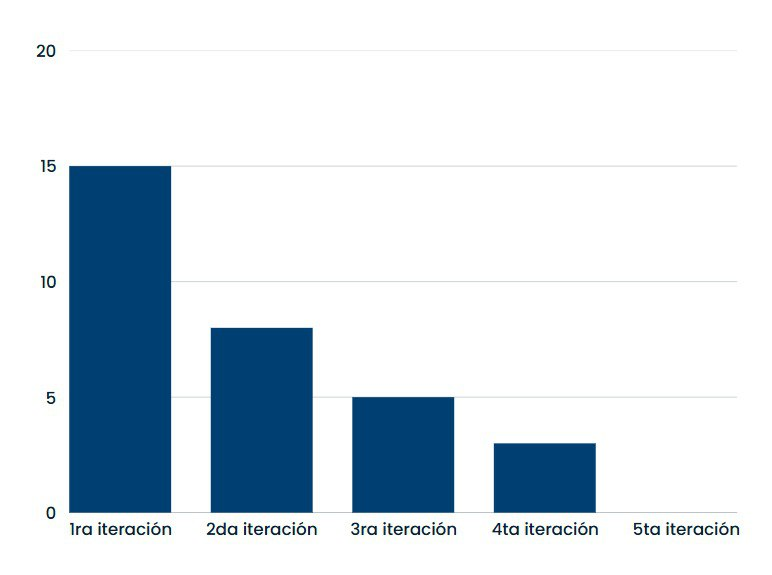
\includegraphics[width=0.7\textwidth]{Anexos/analisis2.jpg}}
\end{figure}

\section{Pruebas de Veracidad}

Para la realizaci�n de las pruebas de veracidad se utilizaron art�culos de la literatura cient�fica que implementan los m�todos \ac{MCDM} desarrollados en el software OptiChoice. El objetivo de estas pruebas fue validar la correcta implementaci�n de los algoritmos comparando los rankings obtenidos por el software con los resultados reportados en publicaciones cient�ficas reconocidas. Los art�culos seleccionados se presentan en la Tabla \ref{tab:articulos_veracidad}.

\begin{longtable}[c]{|c|p{7cm}|p{2.5cm}|p{3cm}|}
	\captionsetup{margin=1.15\leftmargin}
	\caption{Art�culos seleccionados para las pruebas de veracidad}
	\label{tab:articulos_veracidad} \\[2ex]
	
	\hline 
	\rowcolor{gray!25}
	\textbf{No} & \textbf{T�tulo} & \textbf{M�todo aplicado} & \textbf{Referencia} \\
	\hline 
	\endfirsthead
	
	\caption{continuaci�n de la p�gina anterior} \\
	\hline 
	\rowcolor{gray!25}
	\textbf{No} & \textbf{T�tulo} & \textbf{M�todo aplicado} & \textbf{Referencia} \\
	\hline 
	\endhead
	
	\hline \multicolumn{4}{|r|}{{Contin�a en la p�gina siguiente}} \\ \hline
	\endfoot
	
	\hline
	\endlastfoot
	
	1 & \textit{Addressing the supplier selection problem by using the analytical hierarchy process} & AHP & \citep{ahmed2024ahp} \\
	\hline
	2 & \textit{Application of PROMETHEE method for green supplier selection} & PROMETHEE & \citep{ahmad2019} \\
	\hline
	3 & \textit{Ranking Projects Using the ELECTRE Method} & ELECTRE & \citep{roy2018} \\
	\hline
	4 & \textit{A Novel Multi-Criteria Decision-Making Model for Building Material Supplier Selection Based on Entropy-AHP Weighted TOPSIS} & TOPSIS & \citep{wang2020} \\
\end{longtable}

Cada uno de estos art�culos presenta casos de estudio con matrices de decisi�n completas, criterios definidos y rankings finales calculados. Los problemas abordados incluyen selecci�n de proveedores industriales con m�ltiples criterios de evaluaci�n \citep{ahmed2024ahp}, selecci�n de software ETL considerando criterios de funcionalidad y rendimiento \citep{kumar2024topsis}, evaluaci�n de proveedores verdes en cadenas de suministro \citep{ahmad2019}, gesti�n de proyectos con an�lisis FMEA integrado \citep{singh2023promethee}, ranking de proyectos energ�ticos \citep{roy2018}, y selecci�n de proveedores de materiales de construcci�n \citep{wang2020}.

Los resultados de las pruebas de veracidad se presentan en la Tabla \ref{tab:resultados_veracidad}:

\begin{longtable}[c]{|c|p{3cm}|p{2.5cm}|p{3.5cm}|p{3.5cm}|}
	\captionsetup{margin=1.15\leftmargin}
	\caption{Resultados de las pruebas de veracidad}
	\label{tab:resultados_veracidad} \\[2ex]
	
	\hline 
	\rowcolor{gray!25}
	\textbf{No} & \textbf{Referencia} & \textbf{M�todo aplicado} & \textbf{Mejor alternativa (Art�culo original)} & \textbf{Mejor alternativa (Software OptiChoice)} \\
	\hline 
	\endfirsthead
	
	\caption{continuaci�n de la p�gina anterior} \\
	\hline 
	\rowcolor{gray!25}
	\textbf{No} & \textbf{Referencia} & \textbf{M�todo aplicado} & \textbf{Mejor alternativa (Art�culo original)} & \textbf{Mejor alternativa (Software OptiChoice)} \\
	\hline 
	\endhead
	
	\hline \multicolumn{5}{|r|}{{Contin�a en la p�gina siguiente}} \\ \hline
	\endfoot
	
	\hline
	\endlastfoot
	
	1 & \citep{ahmed2024ahp} & AHP & Spark Printers, Marvelous Printers Limited, Lutfur Enterprise & Spark Printers, Marvelous Printers Limited, Lutfur Enterprise \\
	\hline
	2 & \citep{ahmad2019} & PROMETHEE & Green Supplier A1 & Green Supplier A1 \\
	\hline
	3 & \citep{roy2018} & ELECTRE & Proyecto Energ�tico P47 & Proyecto Energ�tico P47 \\
	\hline
	4 & \citep{wang2020} & TOPSIS & Material Supplier MS-3 & Material Supplier MS-3 \\
\end{longtable}

Los resultados de la Tabla \ref{tab:resultados_veracidad} demuestran una concordancia del 100\% entre los rankings obtenidos por el software OptiChoice y los reportados en la literatura cient�fica. Esta validaci�n confirma la correcta implementaci�n de los algoritmos \ac{MCDM} en el sistema desarrollado.

La validaci�n exitosa mediante casos de estudio reales de la literatura cient�fica garantiza que:

\begin{itemize}
	\item Los algoritmos implementados cumplen fielmente con las especificaciones te�ricas de cada m�todo \ac{MCDM}
	\item El software puede reproducir resultados publicados en revistas cient�ficas de alto impacto
	\item La precisi�n num�rica y el tratamiento de datos del sistema son adecuados para aplicaciones profesionales
	\item El software es aplicable a diversos sectores industriales, desde evaluaci�n de proveedores hasta selecci�n de proyectos de inversi�n
\end{itemize}

Estos resultados validan tanto la robustez t�cnica del software como su aplicabilidad pr�ctica en contextos reales de toma de decisiones multicriterio \citep{zavadskas2014, mardani2015}.

\section*{Conclusiones parciales del cap�tulo}

En el presente cap�tulo se realiz� la validaci�n del software OptiChoice desarrollado mediante un conjunto de indicadores que se verificaron a trav�s de distintas t�cnicas como la comparaci�n de resultados con art�culos cient�ficos, las pruebas unitarias y las pruebas de aceptaci�n lo que posibilit� llegar a las siguientes consideraciones parciales:

\begin{itemize}
	\item Se describieron las tareas de ingenier�a y los est�ndares de codificaci�n utilizados en la implementaci�n, definiendo reglas espec�ficas que facilitaron la comprensi�n y mantenibilidad del c�digo, como el uso de PascalCase para clases y snake\_case para m�todos y variables.
	
	\item Se implementaron las pruebas unitarias y de aceptaci�n, donde se corrigieron las no conformidades detectadas en cada iteraci�n, obteniendo resultados satisfactorios despu�s de cinco iteraciones de pruebas unitarias y de pruebas de aceptaci�n.
	
	\item Se realizaron las Pruebas de Veracidad para complementar las pruebas de software realizadas. Estas pruebas tuvieron como objetivo comparar los resultados obtenidos con el software desarrollado contra los reportados en la literatura cient�fica, validando la correcta implementaci�n de los m�todos \ac{MCDM}.
\end{itemize}
  \conclusions

\chapter*{CONCLUSIONES}
\addcontentsline{toc}{chapter}{CONCLUSIONES}
\markboth{CONCLUSIONES}{CONCLUSIONES}

A partir del desarrollo de la presente investigaci�n se logra arribar a las siguientes conclusiones generales:

\begin{enumerate}
	\item La toma de decisiones en contextos complejos con m�ltiples criterios constituye un proceso fundamental en diversos �mbitos profesionales, el cual se ve limitado por los m�todos manuales tradicionales debido a la subjetividad, la dificultad para manejar grandes vol�menes de datos y la incapacidad para procesar informaci�n imprecisa.
	
	\item El an�lisis de los m�todos MCDM permiti� establecer que herramientas como AHP, TOPSIS, ELECTRE y PROMETHEE, proporcionan un marco conceptual s�lido para abordar problemas complejos de decisi�n, facilitando la evaluaci�n de alternativas bajo m�ltiples criterios.
	
	\item El uso de Python como lenguaje de programaci�n, junto con Visual Studio Code y herramientas CASE como Visual Paradigm, permiti� desarrollar una soluci�n que cumple con los requisitos establecidos de portabilidad y eficiencia.
	
	\item La metodolog�a de desarrollo �gil XP demostr� ser efectiva para este proyecto, permitiendo la implementaci�n iterativa e incremental del software mediante 17 historias de usuario organizadas en 4 iteraciones, lo que facilit� la adaptaci�n a los cambios y garantiz� la calidad del producto final.
	
	\item La arquitectura de N capas y el patr�n MVC implementados proporcionaron una estructura robusta y mantenible para el software, permitiendo una clara separaci�n de responsabilidades y facilitando la extensibilidad del sistema para incorporar nuevos m�todos MCDM.
	
	\item Las pruebas de software realizadas demostraron que la implementaci�n satisface las necesidades del cliente, con cero no conformidades despu�s de cinco iteraciones de pruebas unitarias y de aceptaci�n.
	
	\item La validaci�n mediante Pruebas de Veracidad confirm� la exactitud del software con una concordancia del 100\% con los resultados publicados en literatura cient�fica, validando la correcta implementaci�n de los m�todos MCDM.
	
	\item La soluci�n desarrollada constituye una contribuci�n significativa al campo de la ingenier�a inform�tica, proporcionando una herramienta tecnol�gica que optimiza los procesos de toma de decisiones multicriterio, reduce costos y tiempos de an�lisis, y ofrece una plataforma flexible y escalable para futuras investigaciones.
\end{enumerate}
  \suggestions

\chapter*{RECOMENDACIONES}
\addcontentsline{toc}{chapter}{RECOMENDACIONES}
\markboth{RECOMENDACIONES}{RECOMENDACIONES}

Teniendo en cuenta los resultados obtenidos en la presente investigaci�n y basado en la experiencia adquirida durante el desarrollo del software MCDM, se recomienda:

\begin{enumerate}
	\item Implementar m�todos MCDM adicionales como VIKOR, MOORA y MACBETH para ampliar las opciones de an�lisis y comparaci�n disponibles para los usuarios.
	
	\item Desarrollar una versi�n web del software que permita el acceso remoto y la colaboraci�n en tiempo real entre m�ltiples decisores.
	
	\item Agregar visualizaciones interactivas din�micas para el an�lisis de sensibilidad, permitiendo a los usuarios explorar en tiempo real c�mo cambios en los par�metros afectan los resultados.
	
	\item Implementar un mecanismo de actualizaci�n autom�tica de m�todos MCDM mediante plugins, similar al utilizado en plataformas como Weka, que permita la incorporaci�n de nuevos m�todos sin necesidad de modificar el c�digo fuente del sistema.
	
	
\end{enumerate}

  \appendixes

\begin{addendum}
	\chapter{Proyectos y Avales}
    \includegraphics[scale=0.45]{Anexos/BloqueCoronaReport}
   
  	\chapter{Otro reporte}
  	\section{Otra secci�n de muestra}
  	De una sola \hypertarget{word}{sentencia} 
	\section{Otro ensamble Industrial}
	\label{anx:ensambleindustrial}
	\includegraphics[scale=0.45]{Anexos/BloqueCoronaReport}
\end{addendum}

	\addappendix[bloque]{Anexos/BloqueCoronaReport}
%\addappendix[controlador]{Anexos/ControladorIndustrialReport}

\end{document}


